% ============================================================
% Compiler Design Lab Project Report
% VIT Template | A4 | Times New Roman | 1.5 spacing
% Figures are in report_figures/ (upload that folder and vit_logo.jpeg with this file).
% ============================================================
\documentclass[12pt,a4paper]{report}

% ---------- geometry (1.5" left for binding, 1" others) ----------
\usepackage[left=1.5in, right=1in, top=1in, bottom=1in]{geometry}

% ---------- font: Times New Roman equivalent ----------
\usepackage{mathptmx}
\usepackage[T1]{fontenc}

% ---------- spacing ----------
\usepackage{setspace}
\onehalfspacing

% ---------- graphics, tables, code ----------
\usepackage{graphicx}
\usepackage{booktabs}
\usepackage{tabularx}
\usepackage{float}
\usepackage{caption}
\captionsetup{font=footnotesize}

% ---------- listings for source code ----------
\usepackage{listings}
\usepackage{xcolor}
\lstset{
  basicstyle=\ttfamily\footnotesize,
  breaklines=true,
  frame=single,
  numbers=left,
  numberstyle=\tiny\color{gray},
  keywordstyle=\color{blue!70!black},
  commentstyle=\color{green!50!black},
  stringstyle=\color{red!60!black},
  tabsize=4,
  showstringspaces=false
}

% ---------- hyperlinks and formatting ----------
\usepackage[hidelinks]{hyperref}
\usepackage{fancyhdr}
\pagestyle{fancy}
\fancyhf{}
\fancyfoot[C]{\thepage}
\renewcommand{\headrulewidth}{0pt}

\usepackage{parskip}
\setlength{\parindent}{0pt}
\setlength{\parskip}{6pt}
% long file and class names in typewriter type cannot be hyphenated: let lines stretch instead of overflowing
\tolerance=2000
\emergencystretch=3em

% ---------- chapter/section formatting ----------
\usepackage{titlesec}
\titleformat{\chapter}[display]
  {\normalfont\fontsize{16}{20}\bfseries\centering}
  {\MakeUppercase{\chaptertitlename}\ \thechapter}{12pt}
  {\fontsize{16}{20}\bfseries\MakeUppercase}
\titlespacing*{\chapter}{0pt}{-20pt}{20pt}

\titleformat{\section}
  {\normalfont\fontsize{14}{18}\bfseries}
  {\thesection}{1em}{\MakeUppercase}
\titlespacing*{\section}{0pt}{12pt}{6pt}

\titleformat{\subsection}
  {\normalfont\fontsize{12}{15}\bfseries}
  {\thesubsection}{1em}{}
\titlespacing*{\subsection}{0pt}{10pt}{4pt}

\titleformat{\subsubsection}
  {\normalfont\fontsize{12}{15}\bfseries\itshape}
  {\thesubsubsection}{1em}{}
\titlespacing*{\subsubsection}{0pt}{8pt}{4pt}

\usepackage{enumitem}
\usepackage{amsmath}
\setcounter{secnumdepth}{2}
\setcounter{tocdepth}{2}

% a reference in APA form: hanging indent, as in the template
\newcommand{\apa}[1]{\par\hangindent=1.27cm\hangafter=1 #1\par}
\newcommand{\refgroup}[1]{\par\vspace{0.35cm}\noindent\textbf{#1}\par\vspace{0.1cm}}

% ============================================================
\begin{document}

% ==================== COVER PAGE ====================
\thispagestyle{empty}
\begin{center}

\vspace*{0.5cm}

\includegraphics[width=0.45\textwidth]{vit_logo.jpeg}

\vspace{1.2cm}
{\fontsize{16}{20}\selectfont \textbf{BCSE307P COMPILER DESIGN LAB PROJECT}}

\vspace{0.3cm}
{\fontsize{14}{18}\selectfont \textbf{(Slot: G2+TG2)}}

\vspace{1.5cm}
{\fontsize{16}{20}\selectfont \textbf{AUTOMATED LLM/AGENT-GUIDED COMPILER CODE OPTIMIZATION}}

\vspace{2cm}
{\fontsize{12}{15}\selectfont \textbf{Submitted by:}}

\vspace{0.5cm}
\begin{tabular}{|l|l|}
\hline
\textbf{Registration Number} & \textbf{Name} \\
\hline
24BCE2972 & Adarsh Sharma Badhai (Team Leader) \\
\hline
24BAI0345 & Nirupam Raut \\
\hline
\end{tabular}

\vspace{1.5cm}
{\fontsize{12}{15}\selectfont \textbf{Under the guidance of:}}

\vspace{0.3cm}
{\fontsize{12}{15}\selectfont Prof. Mukhtar Ahmad Sofi}

\vspace{1.5cm}
{\fontsize{14}{18}\selectfont \textbf{School of Computer Science and Engineering (SCOPE)}}

\vspace{0.3cm}
{\fontsize{12}{15}\selectfont October 2026}

\end{center}
\newpage

% ==================== ABSTRACT ====================
\thispagestyle{fancy}
\begin{center}
{\fontsize{16}{20}\selectfont \textbf{ABSTRACT}}
\end{center}

\vspace{0.5cm}

\setstretch{1.15}
Standard compilers apply a fixed chain of optimization passes, rarely confirming if a specific transformation actually improved the code's efficiency. We built a fully automated, multi-agent system to optimize Three-Address Code (TAC) dynamically. Instead of a static pipeline, an orchestrator loop analyzes the code, ranks available opportunities, and proposes transformations using either a rule-based engine or a Google Gemini LLM fallback. Two more LLMs are supported behind the same interface: Groq in the cloud, and a local model served by Ollama that works with no internet connection. To guarantee correctness, every proposed change must pass a strict dual-verification gate: differential testing across 25+ input sets and symbolic polynomial equivalence for straight-line logic. If a candidate passes, a static cost model evaluates the precise performance benefit before accepting it. Tested on a dataset of 500 programs spanning seven structural categories, the rule-based agent alone achieved an 82.5\% cost reduction. Integrating Gemini pushed this to 91.5\%, largely by successfully rewriting complex loops and conditionals that standard rules missed. Groq reached 90.9\% and the local model 83.3\%. The dual-verification system successfully blocked all 26 of Gemini's incorrect suggestions, proving that language models can be safely integrated into compiler optimization when constrained by formal equivalence checks, resulting in a zero false-positive rate. It also blocked all 6 incorrect suggestions from Groq and all 113 from the local model, so every run finished with zero false positives.

\setstretch{1.5}
\newpage

% ==================== TABLE OF CONTENTS ====================
\begin{center}
{\fontsize{16}{20}\selectfont \textbf{TABLE OF CONTENTS}}
\end{center}
\vspace{0.5cm}

\renewcommand{\contentsname}{}
% keep the list on the same page as its heading (\tableofcontents would start a new page)
\begingroup
\let\clearpage\relax
\vspace*{-2.5cm}
\tableofcontents
\endgroup
\newpage

% ============================================================
\chapter{INTRODUCTION}

\section{Background}

Compiler optimization sits at the boundary between language semantics and machine performance. Since the 1970s, production compilers have shipped with a fixed menu of transformation passes (constant folding, dead-code elimination, loop-invariant code motion, register allocation, and so on) executed in a hardwired order chosen by the compiler engineers. GCC, for instance, runs over two hundred passes in its \texttt{-O2} pipeline (Stallman et al., 2023). LLVM follows a similar philosophy, chaining dozens of analysis and transform passes into a predetermined sequence (Lattner \& Adve, 2004).

The trouble with a fixed pipeline is that it cannot adapt. A program dominated by redundant subexpressions might benefit from aggressive common-subexpression elimination early on, while a program littered with dead stores would be better served by liveness-based cleanup first. The compiler has no way to reason about which pass to run next, or to judge whether a transformation it just applied actually made things better.

Two lines of research have tried to address this rigidity. The first is superoptimization, pioneered by Massalin in 1987 and later scaled up by the STOKE project (Massalin, 1987; Phothilimthana et al., 2016). Superoptimizers search exhaustively (or stochastically) for the shortest instruction sequence that produces the same output, and they verify candidates through testing or SMT solving. They work well on tiny basic blocks but run into combinatorial walls on anything larger.

The second line comes from the recent wave of large language models applied to code. Codex and Code Llama showed that transformer-based models can generate syntactically correct programs from natural-language descriptions (Chen et al., 2021; Rozi\`ere et al., 2023). Meta's LLM Compiler project trained models specifically on LLVM IR and used them to predict which pass ordering would yield the best binary (Cummins et al., 2024). CompilerGym framed pass selection as a reinforcement-learning problem (Cummins et al., 2022). But all of these treat the compiler as a black box whose knobs are being tuned; none of them propose new code-level transformations and verify them against the original semantics.

Translation validation, introduced by Pnueli, Siegel, and Singerman and later refined by Necula, takes the opposite approach (Necula, 2000; Pnueli et al., 1998). Rather than trusting the compiler, it checks after the fact that the output program is semantically equivalent to the input. The idea is sound, but it has mostly been applied as a post-hoc auditor, not as an online decision-maker that guides the optimization process.

Our project brings these threads together. We build a multi-agent system whose orchestrator loop reasons about what to optimize, delegates the actual transformation to either a rule-based engine or an LLM, verifies every candidate through differential testing and symbolic equivalence, and only commits changes that are verified correct and measurably cheaper. The agent runs autonomously from start to finish; no human touches the intermediate code.

\section{Motivation}

We started this project out of a straightforward frustration: compilers are not transparent about why they apply a particular optimization, and they never explain whether a transformation they skipped might have been worthwhile. For a Compiler Design course, understanding optimization is at least as important as implementing parsing and code generation, yet most course projects stop at the TAC generation stage and never close the loop back to correctness.

Two developments made the idea feasible. First, free LLMs are now easy to reach. Our first prototype used a paid API, which made a 500-program run impractical, so we moved to options that cost nothing: Google Gemini and Groq on their free tiers, and a model that runs on our own laptop through Ollama. The local model also removes the dependence on an internet connection and on a daily quota. Second, differential testing is cheap: running a TAC interpreter on a few hundred input vectors takes a fraction of a second per program, so a brute-force equivalence check fits comfortably inside an iterative loop.

The gap we wanted to fill was the absence of any system that pairs an LLM proposer with a verification gate. LLMs hallucinate; that is well documented. But if every suggestion is tested before it is accepted, the hallucination rate becomes a measurable rejection rate rather than a silent bug rate. We thought that would be an interesting thing to quantify, and the results bore it out: 7.65\% of Gemini's proposals, 1.9\% of Groq's and 57\% of the local model's turned out to be wrong, and the verifier caught all of them.

\section{Scope of the Project}

The project covers the following:
\begin{itemize}[leftmargin=2cm]
  \item A complete front-end pipeline (lexer, recursive-descent parser, AST, TAC generator) for a small C-like language with integers, arithmetic, comparisons, logical operators, \texttt{if}/\texttt{else}, \texttt{while}, \texttt{for}, and \texttt{print}, and a second front end that accepts a subset of real C for the live demo.
  \item A TAC interpreter that can execute programs with user-supplied input variables, including division-by-zero trapping and loop-timeout detection.
  \item Dataflow analyses on the instruction-level control-flow graph: liveness, available copies, and definite assignment.
  \item Six rule-based optimization passes: constant folding, algebraic simplification, dead-code elimination, common-subexpression elimination, strength reduction, and copy propagation.
  \item An Optimization Specialist that routes every step to the rule-based optimizer or to an LLM, in one of three modes (\texttt{rule}, \texttt{hybrid}, \texttt{llm}).
  \item Three LLM proposers behind one interface: Google Gemini, Groq, and a local model served by Ollama for offline use, with structured prompting, response parsing, and automatic retry or disable on API errors.
  \item A two-stage verifier combining differential testing (random, edge, boundary, small-scope and pairwise input sets) and symbolic polynomial equivalence checking.
  \item A weighted static cost model used as the accept/reject gate.
  \item An orchestrator that ties these components into an autonomous loop running up to 50 iterations per program.
  \item A 500-program dataset covering seven structural categories (arithmetic, nested, repeated-expression, dead-code, loops, conditionals, mixed).
  \item Seven visualization charts and a per-program decision log recording every step the agent took, including every routing decision.
\end{itemize}

What the project does not cover:
\begin{itemize}[leftmargin=2cm]
  \item Backend code generation (register allocation, instruction selection, machine code emission).
  \item Interprocedural or whole-program optimization (function inlining, call-graph analysis).
  \item Floating-point arithmetic, arrays or string types.
  \item SMT-based formal verification via Z3 (we rely on differential testing and symbolic equivalence instead).
  \item Measured execution time: the cost model is static.
\end{itemize}


% ============================================================
\chapter{PROJECT DESCRIPTION AND GOALS}

\section{Literature Review}

\subsection{Classical Compiler Optimization}

The Dragon Book (Aho et al., 2006) remains the standard reference for dataflow-driven optimization. It describes the lattice-theoretic framework underpinning constant propagation, liveness analysis, and available-expression analysis, and it lays out the algorithms for dead-code elimination, common-subexpression elimination, and loop-invariant code motion. Our implementation follows the Dragon Book's formulation of liveness and available-copy analysis closely, adapting the iterative fixed-point algorithms to operate at the instruction level rather than the basic-block level.

Muchnick's textbook (Muchnick, 1997) goes deeper into SSA form, partial redundancy elimination, and global value numbering. We did not adopt SSA (our TAC stays in a simpler named-variable form), but Muchnick's treatment of copy propagation and algebraic simplification informed several of our rule-based transformations.

\subsection{Superoptimization and Stochastic Search}

Massalin's 1987 superoptimizer (Massalin, 1987) was the first system to enumerate all possible instruction sequences of increasing length and test each one against the original program. The approach is exact but impractical beyond five or six instructions. STOKE (Phothilimthana et al., 2016) replaced exhaustive search with Markov-chain Monte Carlo sampling, trading completeness for scalability. STOKE verifies candidates using a combination of test-case evaluation and, optionally, an SMT solver. Our differential-testing verifier is conceptually similar to STOKE's test-case phase, though we add symbolic polynomial normalization as a second check.

\subsection{Translation Validation}

Pnueli et al. introduced translation validation as a way to verify each run of a compiler rather than verifying the compiler itself (Pnueli et al., 1998). Necula extended the idea to handle optimizations like loop unrolling and strength reduction by constructing a simulation relation between the source and target programs (Necula, 2000). Our symbolic verifier is a lightweight variant of this idea: it traces both programs symbolically and compares canonical polynomial representations of the printed output expressions.

\subsection{Large Language Models for Code Transformation}

Codex (Chen et al., 2021) demonstrated that language models trained on code can solve programming problems with surprisingly high accuracy. Code Llama (Rozi\`ere et al., 2023) extended this to open-weight models fine-tuned on code-heavy corpora. More recently, Meta's LLM Compiler (Cummins et al., 2024) fine-tuned Code Llama on 546 billion tokens of LLVM IR and assembly, training it to predict optimized IR and optimal pass orderings. CompilerGym (Cummins et al., 2022) framed compiler optimization as a reinforcement-learning environment. Our work differs from these in a fundamental way: we use the LLM not to pick a pass ordering but to directly propose a rewritten TAC program, and we verify the proposal before accepting it. Open-weight code models can also be run locally (Ollama, 2026), which lets the same proposer work with no internet connection.

\subsection{Multi-Agent Architectures}

AutoGen (Wu et al., 2023) showed that multi-agent conversations, where different agents take on different roles, can solve complex tasks more reliably than a single monolithic prompt. CrewAI and similar frameworks have since popularized the pattern for code generation and research workflows. Our orchestrator--specialist architecture borrows from this idea: the orchestrator does not itself know how to fold constants or eliminate dead code; it delegates to specialist agents and arbitrates their output through the verifier and cost evaluator.

\section{Gaps Identified}

After surveying the literature, we identified the following gaps:
\begin{enumerate}[leftmargin=2cm]
  \item Classical compilers do not reason about which pass to apply next or whether a transformation was actually beneficial. The pass ordering is hardwired.
  \item Superoptimizers handle small code fragments well but cannot scale to programs with loops and branches.
  \item LLM-based code tools produce plausible output but provide no correctness guarantee. An LLM can silently change program semantics, and the user has no way to know without manual inspection.
  \item Existing LLM-compiler work focuses on pass ordering or flag selection, not on proposing new code-level transformations.
  \item No prior system combines an LLM-based transformation proposer with a formal or semi-formal verification gate that blocks incorrect suggestions automatically.
  \item LLM-based tools usually depend on one cloud provider: without a connection, a key or remaining quota they stop working.
\end{enumerate}

\section{Objectives}

\begin{enumerate}[leftmargin=2cm]
  \item Build a multi-agent architecture with five clearly separated components: an orchestrator, a code analysis specialist, an optimization specialist (rule-based and LLM-based), a verification module, and a cost evaluator.
  \item Implement the orchestrator loop: analyze, propose, verify, evaluate, accept or reject, and repeat until no opportunity remains.
  \item Detect six types of optimization opportunities (constant folding, algebraic simplification, dead-code elimination, common-subexpression elimination, strength reduction, copy propagation) and apply the highest-priority one at each step.
  \item Implement dual verification: differential testing on many input sets and symbolic polynomial equivalence for straight-line code.
  \item Accept a transformation only when both verification and cost evaluation confirm it is correct and beneficial.
  \item Integrate free LLMs (Google Gemini and Groq) as proposers, with the same verification gates as rule-based proposals, and let one component decide for every step whether the rules or the LLM should propose.
  \item Keep the system usable with no internet connection by supporting a local model.
  \item Run the agent on 500 programs across seven categories and report verification pass rate, acceptance rate, cost reduction, convergence steps, LLM validity rate, and false-positive rate.
  \item Produce seven visualization charts summarizing the agent's behavior across the dataset.
\end{enumerate}

\section{Problem Statement}

Given a program written in a C-like source language, automatically lower it to Three-Address Code and then iteratively optimize the TAC through an autonomous agent loop that (a) identifies optimization opportunities using dataflow analysis, (b) proposes a single transformation per iteration, either rule-based or LLM-generated, as decided by a router, (c) verifies the candidate against the current program through differential testing and symbolic equivalence, (d) accepts the change only if the weighted cost strictly decreases, and (e) repeats until convergence. The system must achieve an average cost reduction above 30\% across a 500-program dataset, with a false-positive rate of exactly zero, and it must keep working when no LLM can be reached.

\section{Project Plan}

\begin{table}[H]
\centering
\caption{Project timeline and milestones}
\label{tab:plan}
\begin{tabularx}{\textwidth}{|c|X|l|}
\hline
\textbf{Phase} & \textbf{Task} & \textbf{Duration} \\
\hline
1 & Literature survey; define source language grammar; design TAC instruction set & Weeks 1--2 \\
\hline
2 & Implement lexer, parser, AST, TAC generator, and TAC interpreter & Weeks 3--4 \\
\hline
3 & Implement dataflow analyses (CFG, liveness, available copies, definite assignment) & Week 5 \\
\hline
4 & Build the five agent components (analyzer, rule optimizer, verifier, cost evaluator, decision logger) & Weeks 5--7 \\
\hline
5 & Wire agents into the orchestrator loop; run on small test programs; debug & Week 7 \\
\hline
6 & Generate the 500-program dataset; run the rule-based agent on all programs; collect metrics & Week 8 \\
\hline
7 & Integrate Google Gemini LLM proposer; run the combined agent; compare with rule-only baseline & Week 9 \\
\hline
8 & Build visualization charts; write decision-log exporter & Weeks 9--10 \\
\hline
9 & Add the Optimization Specialist router; add the Groq and Ollama backends and the offline mode & Week 11 \\
\hline
10 & Test the verifier itself (fuzzing, mutation testing); add small-scope and pairwise input sets & Week 12 \\
\hline
11 & Full runs with all three LLMs; C front end and live demo; report & Weeks 12--13 \\
\hline
\end{tabularx}
\end{table}


% ============================================================
\chapter{TECHNICAL SPECIFICATION}

\section{Requirements}

\subsection{Functional Requirements}

\begin{enumerate}[leftmargin=2cm]
  \item \textbf{Source-to-TAC compilation:} The system shall accept programs written in the defined C-like language and produce correct Three-Address Code through lexing, parsing, and code generation.
  \item \textbf{Optimization opportunity detection:} The code analyzer shall identify constant-folding, algebraic-simplification, dead-code-elimination, common-subexpression, strength-reduction, and copy-propagation opportunities from the TAC, using dataflow analysis on the instruction-level control-flow graph.
  \item \textbf{Routing and transformation proposal:} The Optimization Specialist shall route each step to the rule-based optimizer or to an LLM and record the reason. The rule-based optimizer shall apply exactly one transformation per iteration. The LLM optimizer shall, when invoked, send the current TAC to the configured model (Gemini, Groq or a local Ollama model) and parse the returned candidate.
  \item \textbf{Dual verification:} Every candidate (rule-based or LLM-generated) shall pass differential testing on at least 25 input sets and, for straight-line code, symbolic polynomial equivalence checking, before being considered for acceptance.
  \item \textbf{Cost-based acceptance:} A candidate shall be accepted only if its weighted static cost is strictly lower than the current program's cost.
  \item \textbf{Iterative convergence:} The orchestrator shall repeat the loop until no opportunity remains or the iteration cap (50) is reached.
  \item \textbf{Decision logging:} Every iteration shall be logged with the opportunity analyzed, the route chosen, the transformation proposed, the verification outcome, the cost change, and the accept/reject decision. Logs shall be saved in both human-readable text and structured JSON.
  \item \textbf{Metrics and visualization:} The system shall compute verification pass rate, acceptance rate, average cost reduction, convergence steps, LLM validity rate, and false-positive count, and produce seven charts.
\end{enumerate}

\subsection{Non-Functional Requirements}

\begin{enumerate}[leftmargin=2cm]
  \item \textbf{Correctness guarantee:} The false-positive rate must be exactly 0\%. No incorrectly optimized program shall pass the verification gate.
  \item \textbf{Modularity:} Each agent component shall be a separate Python class with a documented input/output interface, so that new optimizations, verification methods or LLM providers can be added without modifying other components.
  \item \textbf{Performance:} A single program shall be optimized in well under a second with the rules alone and in a few seconds with a cloud LLM. The full 500-program dataset shall complete in under 3 minutes without an LLM and in under 45 minutes with a cloud LLM.
  \item \textbf{Graceful degradation:} If the LLM is unavailable (missing key, quota exhaustion, network failure, local server stopped), the system shall fall back to rule-based optimization and log the reason.
  \item \textbf{Offline operation:} The whole agent, including an LLM proposer, shall be able to run with no internet connection.
  \item \textbf{Reproducibility:} The dataset generator shall produce identical programs when run with the same parameters. Metrics and logs shall be saved in machine-readable formats.
\end{enumerate}

\section{System Specification}

\subsection{Hardware Specification}

\begin{table}[H]
\centering
\caption{Hardware configuration used for development and testing}
\label{tab:hardware}
\begin{tabularx}{\textwidth}{|l|X|}
\hline
\textbf{Component} & \textbf{Specification} \\
\hline
Processor & Intel Core i5 / AMD Ryzen 5 or equivalent (the runs were made on a 13th-generation Intel Core i5 laptop) \\
\hline
RAM & 8 GB minimum; 16 GB for the local model \\
\hline
Storage & 500 MB free disk space; a further 4.7 GB for the local model \\
\hline
Network & Internet connection for the Gemini and Groq calls only; none in offline mode \\
\hline
\end{tabularx}
\end{table}

\subsection{Software Specification}

\begin{table}[H]
\centering
\caption{Software stack}
\label{tab:software}
\begin{tabularx}{\textwidth}{|l|l|X|}
\hline
\textbf{Software} & \textbf{Version} & \textbf{Purpose} \\
\hline
Python & 3.10+ & Core language (uses \texttt{match} statements) \\
\hline
google-genai & $\geq$1.0 & Gemini API client \\
\hline
Groq API & HTTP & Called with the Python standard library; no package needed \\
\hline
Ollama & 0.40 & Local model server, with the model \texttt{qwen2.5-coder:7b} \\
\hline
matplotlib & $\geq$3.8 & Bar, line, scatter, heatmap charts \\
\hline
plotly & $\geq$5.18 & Interactive Sankey diagram \\
\hline
seaborn & $\geq$0.13 & Heatmap styling \\
\hline
numpy & $\geq$1.26 & Trend-line computation \\
\hline
kaleido & $\geq$0.2.1 & Plotly PNG export \\
\hline
pytest & $\geq$8.0 & Unit and integration testing \\
\hline
\end{tabularx}
\end{table}


% ============================================================
\chapter{DESIGN APPROACH AND DETAILS}

\section{Datasets}

We wrote a Python generator (\texttt{dataset/generator.py}) that creates 500 source programs spread across seven categories. Each category targets a different mix of optimization opportunities, so the agent faces a range of challenges rather than the same pattern repeated.

\begin{table}[H]
\centering
\caption{Dataset composition}
\label{tab:dataset}
\begin{tabularx}{\textwidth}{|l|c|X|}
\hline
\textbf{Category} & \textbf{Count} & \textbf{What it tests} \\
\hline
Arithmetic-only & 60 & Straight-line constant expressions (\texttt{int k = 1 + 14}) \\
\hline
Nested expressions & 60 & Multi-level parenthesized sub-expressions requiring many temporaries \\
\hline
Repeated expressions & 60 & Identical sub-expressions computed more than once (CSE targets) \\
\hline
Dead code & 60 & Variables assigned but never read or printed \\
\hline
Loops & 80 & \texttt{for}/\texttt{while} loops with loop-invariant computations and dead stores inside the body \\
\hline
Conditionals & 80 & \texttt{if}/\texttt{else} branches with algebraic identities (\texttt{x * 1}, \texttt{x + 0}) \\
\hline
Mixed & 100 & Programs combining two or more of the above in a single source file \\
\hline
\end{tabularx}
\end{table}

Programs that use input variables (read-before-write) list them in an \texttt{// inputs:} header comment. The verifier feeds those variables many different values during differential testing. Programs without input variables have exactly one possible execution, so a single test run constitutes a proof of equivalence.

\section{System Architecture}

Figure~\ref{fig:architecture} shows the architecture. Source code enters at the top left, passes through the front end (lexer, parser, AST, TAC generator), and arrives at the agent loop. The Orchestrator controls the cycle: it asks the Code Analysis Specialist to scan the TAC, hands the step to the Optimization Specialist, which routes it to the rules or to an LLM, has the candidate verified, has its cost evaluated, and decides whether to accept. The loop repeats until nothing is left to try. The run then ends with a final check of the optimized program against the original, and its outputs are the optimized TAC, the per-program decision log, the metrics files and the charts.

\begin{figure}[H]
\centering
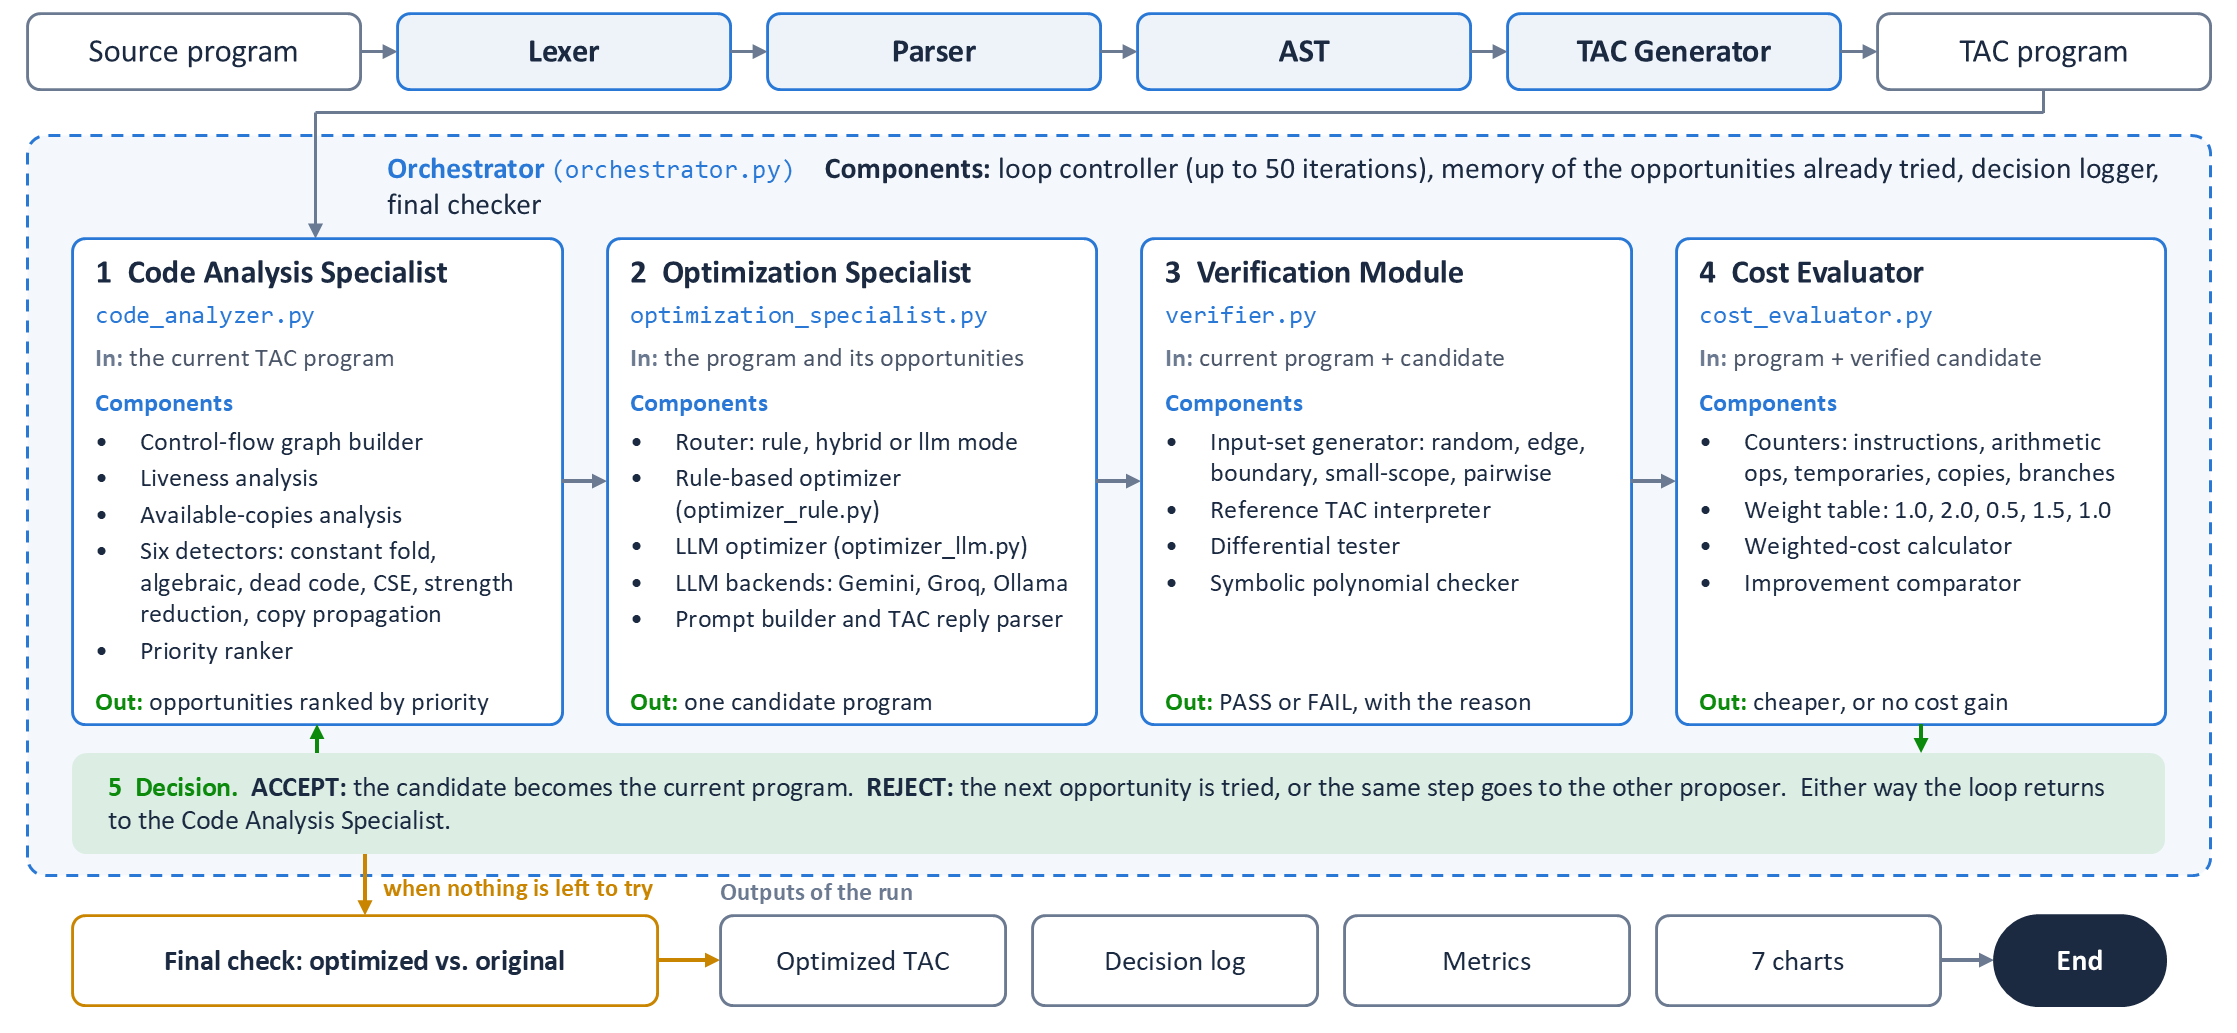
\includegraphics[width=\textwidth]{report_figures/architecture.png}
\caption{System architecture: the front end, the agent loop with the components of each agent, and the end of a run}
\label{fig:architecture}
\end{figure}

\begin{itemize}[leftmargin=2cm]
  \item \textbf{Orchestrator.} Runs the loop for up to 50 iterations per program, remembers which opportunities were already turned down, logs every decision, and re-verifies the final program against the untouched original.
  \item \textbf{Code Analysis Specialist.} Builds the control-flow graph, runs the liveness and available-copies analyses, and returns the opportunities it finds, ranked by priority (constant folding 100, algebraic simplification 90, dead code 80, CSE 70, strength reduction 60, copy propagation 50).
  \item \textbf{Optimization Specialist.} Decides who proposes the next change and returns one candidate program. Option A is the rule-based optimizer, which applies the highest-priority opportunity to a copy of the program. Option B is an LLM, which receives the TAC and is asked for one semantics-preserving optimization.
  \item \textbf{Verification Module.} Runs the current program and the candidate on the same inputs and compares printed output and failure mode; for straight-line code it also checks symbolic equivalence.
  \item \textbf{Cost Evaluator.} Computes the weighted cost of both programs and accepts the change only if the cost strictly drops.
\end{itemize}

\subsection{Routing Between the Rules and the LLM}

The Optimization Specialist has three routing modes, listed in Table~\ref{tab:routing}. Whatever the route, the proposal goes through the same verification and cost gates. The LLM is never asked about a program that is already nothing but constant \texttt{print} instructions, because that form is provably minimal. Every routing decision is written to the decision log together with its reason.

\begin{table}[H]
\centering
\caption{Routing modes of the Optimization Specialist}
\label{tab:routing}
\begin{tabularx}{\textwidth}{|l|l|X|}
\hline
\textbf{Mode} & \textbf{First choice} & \textbf{Falls back to the other proposer when} \\
\hline
\texttt{rule} & Rules & Never: the LLM is not used \\
\hline
\texttt{hybrid} & Rules & The rule proposal for the step was turned down, or the rules have nothing left to try \\
\hline
\texttt{llm} & LLM & The LLM is not running, its call budget is used up, or its proposal was turned down \\
\hline
\end{tabularx}
\end{table}

\subsection{LLM Backends}

All three backends share one prompt and one reply parser, so their results are directly comparable (Table~\ref{tab:backends}). The provider is chosen automatically: Gemini, then Groq, then Ollama, whichever is configured and reachable. An offline switch forces the local model.

\begin{table}[H]
\centering
\caption{The three LLM backends}
\label{tab:backends}
\small
\begin{tabularx}{\textwidth}{|l|l|l|X|}
\hline
\textbf{Backend} & \textbf{Model} & \textbf{Runs on} & \textbf{Notes} \\
\hline
Gemini & \texttt{gemini-3.1-flash-lite} & Google cloud & Free API key; called through the SDK \\
\hline
Groq & \texttt{gpt-oss-120b} & Groq cloud & Free API key; moves to the next model when a daily quota is spent \\
\hline
Ollama & \texttt{qwen2.5-coder:7b} & The laptop & No key and no internet; falls back to the CPU if the GPU runner fails \\
\hline
\end{tabularx}
\end{table}

\section{Algorithms}

The project relies on several well-known compiler algorithms, each adapted to work on individual TAC instructions rather than basic blocks.

\subsection{Liveness Analysis (Backward May-Analysis)}

Starting from the last instruction, we propagate live variable sets backward through the CFG. At each instruction, a variable is added to the live set if it is read, and removed if it is defined. The analysis iterates until no set changes. Dead-code elimination uses the resulting live-out sets: if an instruction defines a variable that is not live at its exit and cannot trap (no division by a variable), the instruction is dead.

\subsection{Available-Copy Analysis (Forward Must-Analysis)}

We track pairs $(x, y)$ meaning ``$x = y$ is still valid.'' At CFG joins we intersect, so a copy is available only if it reaches along every path. Whenever $x$ or $y$ is redefined, all pairs mentioning it are killed. Copy propagation uses these sets to replace uses of $x$ with $y$ wherever the copy is available.

\subsection{Symbolic Polynomial Normalization}

For straight-line code (no labels, no jumps), we trace each variable as a multivariate polynomial in the input variables. Addition, subtraction, and multiplication map directly to polynomial operations, so $x + x$ and $2 \times x$ normalize to the same polynomial; division and modulo produce opaque terms that are compared structurally. Two programs are symbolically equivalent if their printed expressions normalize to the same polynomial, and the set of divisors that could trap before each print is identical.

\subsection{Differential Testing}

We run the current and the candidate TAC programs through the interpreter on the same input sets. Both programs must print the same output sequence and either both succeed or both fail with the same exception type (such as a division by zero or a timeout). The input sets are built in five ways, listed in Table~\ref{tab:inputs}.

\begin{table}[H]
\centering
\caption{Input sets used by differential testing}
\label{tab:inputs}
\begin{tabularx}{\textwidth}{|l|X|l|}
\hline
\textbf{Input sets} & \textbf{What is tried} & \textbf{What it catches} \\
\hline
Random & 20 sets with values from $-100$ to $100$ & General differences \\
\hline
Edge cases & All inputs equal to 0, 1, $-1$, 99, $-99$ & Zero and sign handling \\
\hline
Boundary & $c-1$, $c$, $c+1$ for every literal $c$ & Off-by-one comparisons \\
\hline
Small scope & Every combination of a few small values (one input: every value from $-128$ to $128$) & \texttt{\&\&} against \texttt{||}, a branch on a flag \\
\hline
Pairwise & Every two inputs with every two boundary values & Two inputs that must line up \\
\hline
\end{tabularx}
\end{table}

The last two kinds were added after mutation testing (Section~\ref{sec:testing}) showed that random values almost never make one input zero while another is not, which is exactly what tells \texttt{\&\&} from \texttt{||}.

\section{Design}

\subsection{Data Flow Diagram}

\begin{figure}[H]
\centering
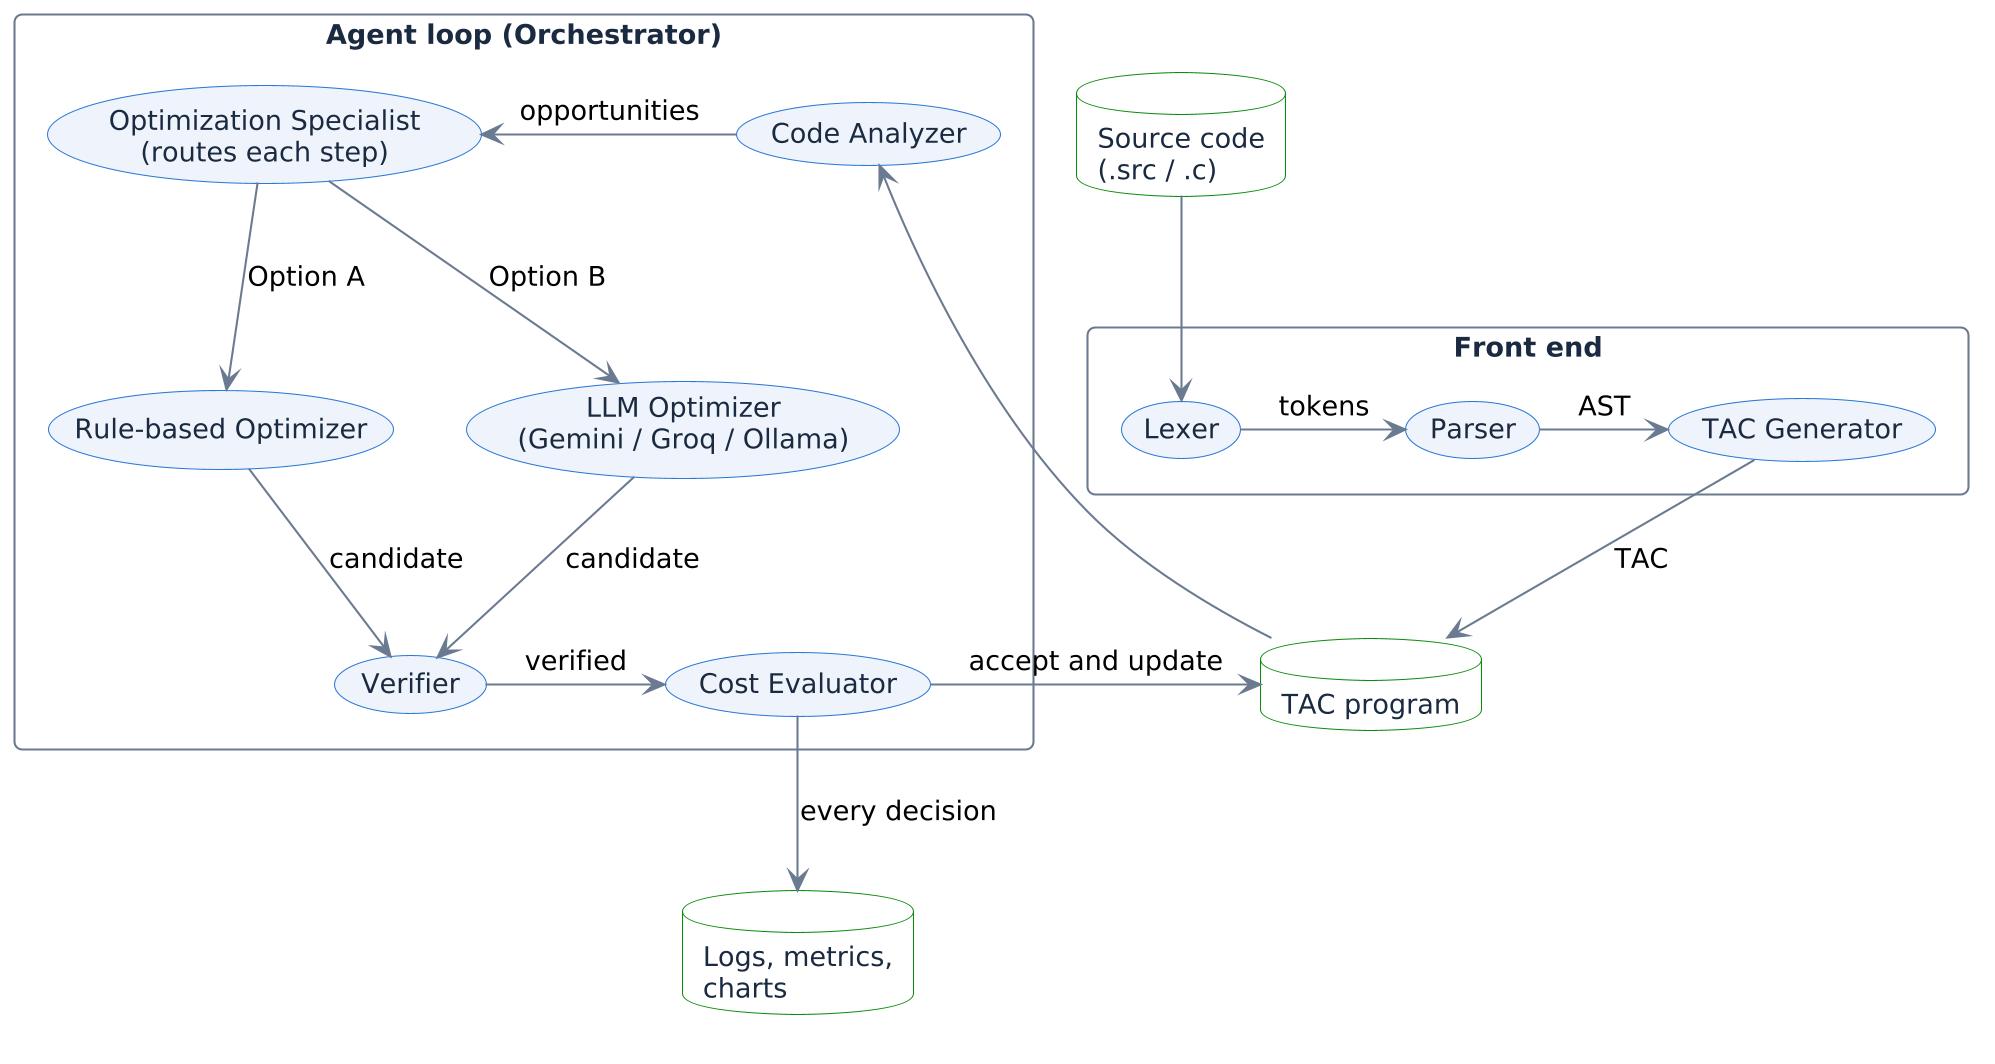
\includegraphics[width=\textwidth]{report_figures/data_flow.png}
\caption{Data flow diagram showing inputs, outputs, and intermediate data at each stage}
\label{fig:dfd}
\end{figure}

\subsection{Class Diagram}

\begin{figure}[H]
\centering
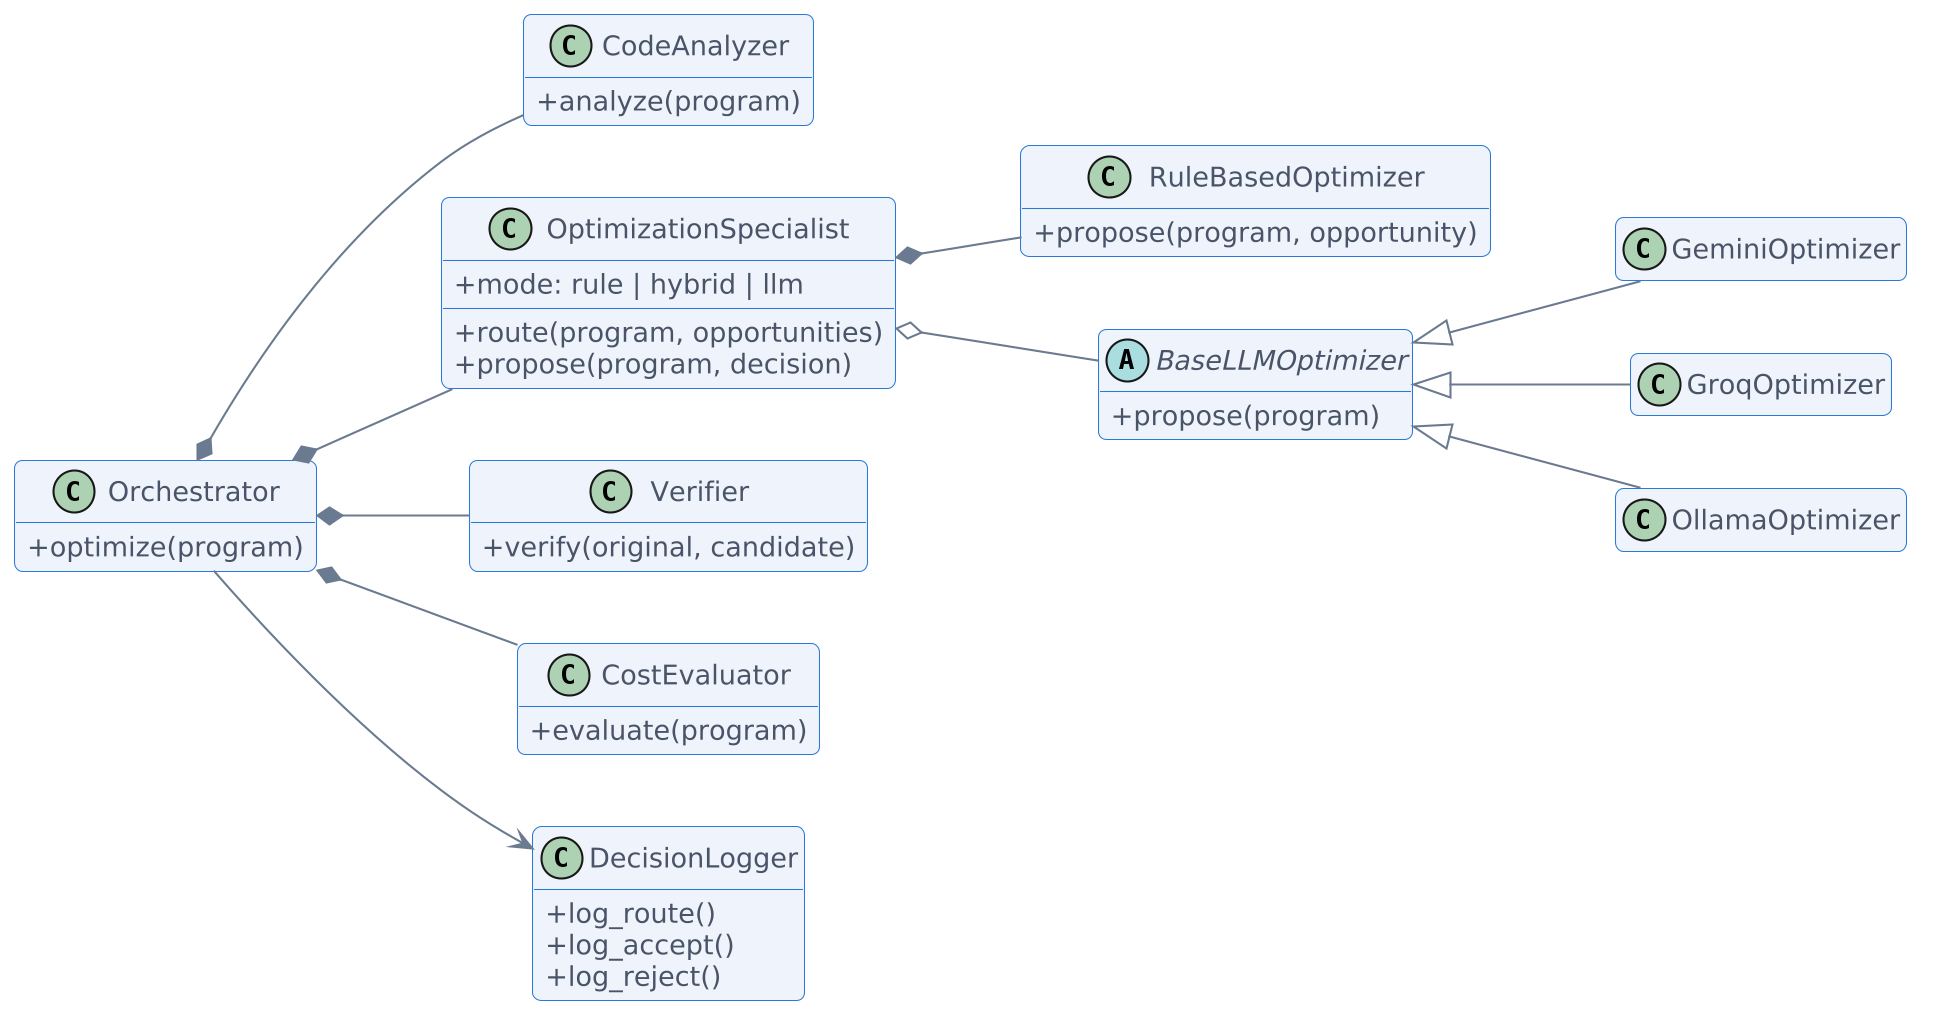
\includegraphics[width=\textwidth]{report_figures/class_diagram.png}
\caption{Class diagram of the agent architecture. The Optimization Specialist owns the rule-based optimizer and holds one of three interchangeable LLM backends}
\label{fig:class}
\end{figure}


% ============================================================
\chapter{IMPLEMENTATION}

This chapter walks through the major modules, shows representative code fragments, and describes the test suite. All source code is in Python 3.10+.

\section{Module Description}

\subsection{Module 1: Front End (\texttt{src/frontend/})}

The front end has four files: \texttt{lexer.py} (tokenization), \texttt{ast\_nodes.py} (AST dataclasses), \texttt{parser.py} (recursive-descent parser), and \texttt{tac\_generator.py} (AST-to-TAC lowering). A convenience function \texttt{compile\_source(text)} chains the stages. A second front end, \texttt{c\_frontend.py}, parses a subset of real C into the same AST, so an ordinary \texttt{.c} file can go through the same agents in the live demo.

\begin{lstlisting}[language=Python, caption={From \texttt{tac\_generator.py}: lowering an if statement that has an else part to TAC (trimmed)}, label=lst:genif]
def _gen_if(self, stmt: IfStmt) -> None:
    cond = self._gen_expr(stmt.condition)
    l_else = self._new_label()
    l_end = self._new_label()
    self._emit(TACInstruction(TACOp.IF_FALSE_GOTO, arg1=cond, label=l_else))
    self._gen_block(stmt.then_body)
    self._emit(TACInstruction(TACOp.GOTO, label=l_end))
    self._emit(TACInstruction(TACOp.LABEL, label=l_else))
    self._gen_block(stmt.else_body)
    self._emit(TACInstruction(TACOp.LABEL, label=l_end))
\end{lstlisting}

\subsection{Module 2: TAC Representation and Interpreter (\texttt{src/tac/})}

The TAC subsystem defines \texttt{TACInstruction} (a dataclass with fields \texttt{op}, \texttt{result}, \texttt{arg1}, \texttt{operator}, \texttt{arg2}), \texttt{TACProgram} (a container with serialization, deep copy, and input-variable detection), and \texttt{TACInterpreter} (an execution engine that returns printed output as a list of integers). The interpreter enforces C-style truncating division and raises typed exceptions (\texttt{DivisionByZeroError}, \texttt{ExecutionTimeout}, \texttt{UndefinedVariableError}) that the verifier distinguishes when comparing runs.

\texttt{dataflow.py} holds the CFG builder and the analyses: liveness, available copies, definite assignment, and reachability. All follow the textbook iterative fixed-point pattern.

\subsection{Module 3: Agent Components (\texttt{src/agents/})}

The five components are separate classes. \texttt{orchestrator.py} runs the loop; \texttt{code\_analyzer.py} finds opportunities; \texttt{optimization\_specialist.py} routes each step and owns \texttt{optimizer\_rule.py} and \texttt{optimizer\_llm.py}; \texttt{verifier.py} and \texttt{cost\_evaluator.py} are the two gates. Listing~\ref{lst:orch} is the core logic of the Orchestrator. It enforces our safety rules: a change is only kept if it passes verification \emph{and} reduces the static cost. If the proposal for a step is turned down, the Specialist may hand the same step to the other proposer.

\begin{lstlisting}[language=Python, caption={The Orchestrator loop (trimmed, from \texttt{orchestrator.py})}, label=lst:orch]
for iteration in range(1, self.max_iterations + 1):
    # 1. ANALYZE (leaving out opportunities already turned down)
    opportunities = [o for o in self.analyzer.analyze(current)
                     if self._opportunity_key(o) not in attempted]

    # 2-5. PROPOSE -> VERIFY -> EVALUATE -> ACCEPT/REJECT
    tried, outcome = [], None
    while outcome not in ("accepted", "unverifiable"):
        decision = specialist.route(current, opportunities,
                                    llm_calls, tried)
        if decision.route is None:
            break                    # nobody can propose anything more
        tried.append(decision.route)
        proposal = specialist.propose(current, decision, opportunities)
        outcome = self._judge(iteration, current, proposal)
        if outcome == "accepted":
            current = proposal.candidate
            attempted.clear()        # new opportunities may appear

    if outcome != "accepted" and not opportunities:
        break                        # converged: nothing left to try
\end{lstlisting}

The verifier (\texttt{verifier.py}, 386 lines) runs differential testing first. If the program has no control flow, it also runs the symbolic trace and requires both to agree. The cost evaluator (\texttt{cost\_evaluator.py}, 64 lines) counts instructions, arithmetic operations, temporary variables, memory operations (copies), and branch operations, multiplies each by a fixed weight (1.0, 2.0, 0.5, 1.5 and 1.0), and sums them into a single scalar.

\subsection{Module 4: Optimization Specialist and Routing}

The routing decision is a short method of the Optimization Specialist (Listing~\ref{lst:route}). The mode sets the order in which the two proposers are considered, and a proposer is skipped when it has nothing to offer.

\begin{lstlisting}[language=Python, caption={The routing decision (trimmed, from \texttt{optimization\_specialist.py})}, label=lst:route]
def route(self, program, opportunities, llm_calls=0, tried=()):
    order = ([Route.RULE, Route.LLM] if self.mode != "llm"
             else [Route.LLM, Route.RULE])
    if not self.llm_attached:
        order = [Route.RULE]
    passed_over, llm_note = [], ""
    for route in order:
        if route in tried:
            name = "rule-based" if route is Route.RULE else "LLM"
            passed_over.append(f"the {name} proposal was turned down")
        elif route is Route.RULE and not opportunities:
            passed_over.append("the rules have nothing left to try")
        elif route is Route.LLM and (
                llm_note := self._llm_blocker(program, llm_calls)):
            passed_over.append(f"LLM not used, {llm_note}")
        else:
            reason = self._reason(route, opportunities, passed_over)
            return RoutingDecision(route, reason, llm_note)
    return RoutingDecision(None, "; ".join(passed_over), llm_note)
\end{lstlisting}

\subsection{Module 5: LLM Optimizer (\texttt{src/agents/optimizer\_llm.py})}

The LLM optimizer defines a base class \texttt{BaseLLMOptimizer} with a shared prompt template and response parser, and three concrete subclasses: \texttt{GeminiOptimizer} calls the Google Gen AI SDK, \texttt{GroqOptimizer} calls Groq's HTTP API and moves to the next model when a daily quota is spent, and \texttt{OllamaOptimizer} calls a model running on the same machine. The prompt asks the model to propose ``exactly one semantics-preserving optimization'' and return the result inside \texttt{<tac>} tags. The parser strips markdown fences and line-number prefixes before feeding the text to \texttt{TACProgram.from\_string()}.

The first prototype also had a provider for a paid API. It was removed, because a paid key made large-scale runs impractical; the three providers that remain are all free to use.

\subsection{Module 6: Visualization and Demo}

\texttt{charts.py} produces seven chart types: (1) Sankey diagram of proposal flow, (2) grouped bar chart of outcomes per optimization type, (3) line chart of cost trajectory for five representative programs, (4) donut chart of accepted optimization types, (5) scatter plot of agent steps vs.\ cost improvement with trend lines, (6) heatmap of category vs.\ optimization type, and (7) a comparison bar chart of rule-only vs.\ rule+LLM reduction per category. \texttt{report.py} aggregates per-program results into the metrics summary (JSON and CSV) and formats the human-readable metrics table. \texttt{demo.py} is a terminal front end that takes a C program and walks through the whole pipeline on screen, stage by stage.

\section{Testing}
\label{sec:testing}

We wrote 336 automated tests across fifteen test files, covering every component (Table~\ref{tab:tests}). The LLM backends are tested against stand-in local servers, so the tests need no API key, no Ollama installation and no network.

\begin{table}[H]
\centering
\caption{Test suite summary}
\label{tab:tests}
\small
\begin{tabular}{|l|l|c|}
\hline
\textbf{Test file} & \textbf{Component} & \textbf{Tests} \\
\hline
\texttt{test\_lexer.py} & Lexer & 14 \\
\hline
\texttt{test\_parser.py} & Parser & 22 \\
\hline
\texttt{test\_tac\_generator.py} & TAC generator & 14 \\
\hline
\texttt{test\_c\_frontend.py} & C front end & 43 \\
\hline
\texttt{test\_interpreter.py} & TAC interpreter & 33 \\
\hline
\texttt{test\_analyzer.py} & Code analyzer & 21 \\
\hline
\texttt{test\_optimizer.py} & Rule and LLM optimizers & 27 \\
\hline
\texttt{test\_optimization\_specialist.py} & Routing & 20 \\
\hline
\texttt{test\_groq.py} & Groq backend & 26 \\
\hline
\texttt{test\_ollama.py} & Ollama backend & 24 \\
\hline
\texttt{test\_verifier.py} & Verifier & 40 \\
\hline
\texttt{test\_cost\_evaluator.py} & Cost evaluator & 10 \\
\hline
\texttt{test\_orchestrator.py} & Orchestrator (integration) & 16 \\
\hline
\texttt{test\_demo.py} & Demo front end & 13 \\
\hline
\texttt{test\_bugfixes.py} & Regression tests & 13 \\
\hline
\end{tabular}
\end{table}

The verifier tests are worth calling out specifically. We inject incorrect transformations (wrong constant folds, operand swaps on non-commutative operators, deletion of live stores, off-by-one loop conditions, removed loop increments, deleted trapping divisions, reordered output, and dropped output) and confirm that every one is rejected. This is how we verify the verifier itself. We then tested the system at a larger scale:

\begin{itemize}[leftmargin=2cm]
  \item \textbf{Fuzzing the rules.} 5,100 random TAC programs were generated, and all 20,968 rule-based proposals for them were compared with the original on inputs the verifier does not use. None changed the program's behaviour.
  \item \textbf{Mutation testing the verifier.} Random branching programs were changed in one place (an operator, a constant or an operand), the way a wrong LLM proposal might be. Of the first 400 mutants, the verifier accepted 194, and 13 of those behaved differently from the original. After the small-scope and pairwise input sets were added, the verifier accepted 351 of 800 mutants and none of them behaves differently.
  \item \textbf{Re-checking the results.} For every run, each final program was executed against its original on every combination of small input values plus random ones (about 64,000 executions per run). No mismatch was found.
  \item \textbf{Replaying the Gemini run.} The 383 recorded Gemini replies were replayed through the strengthened verifier. Every proposal received the same decision as before.
\end{itemize}

The same testing found one bug in the rules: strength reduction rewrote $x \times 2^k$ to a shift even for $k > 64$, which the interpreter rejects. The proposal was caught by the verifier every time, and the analyzer no longer makes it.


% ============================================================
\chapter{RESULTS AND DISCUSSION}

\section{Detailed Results}

We ran the agent four times on the full 500-program dataset: once with the rule-based optimizer only, and three times in \texttt{hybrid} mode, in which an LLM is asked when the rules hit a wall. Table~\ref{tab:metrics} summarizes the headline numbers.

\begin{table}[H]
\centering
\caption{Aggregate metrics across 500 programs}
\label{tab:metrics}
\small
\setlength{\tabcolsep}{4pt}
\begin{tabular}{|l|c|c|c|c|}
\hline
\textbf{Metric} & \textbf{Rule-only} & \textbf{Rule + Gemini} & \textbf{Rule + Groq} & \textbf{Rule + Ollama} \\
\hline
Total proposals & 10,628 & 10,978 & 11,085 & 10,805 \\
\hline
Accepted & 10,517 & 10,828 & 10,925 & 10,579 \\
\hline
Verification pass rate & 100.00\% & 99.76\% & 99.95\% & 98.95\% \\
\hline
Acceptance rate (of verified) & 98.96\% & 98.87\% & 98.61\% & 98.94\% \\
\hline
Avg. cost reduction & 82.49\% & 91.50\% & 90.89\% & 83.28\% \\
\hline
Steps to convergence (mean) & 22.2 & 22.7 & 22.9 & 22.3 \\
\hline
LLM validity rate & --- & 92.35\% & 98.11\% & 42.93\% \\
\hline
False positives & \textbf{0} & \textbf{0} & \textbf{0} & \textbf{0} \\
\hline
\end{tabular}
\end{table}

The rule-based agent already meets the 30\% cost-reduction target for every single program. Adding a cloud LLM lifts the average by roughly nine percentage points, with the biggest gains in the categories that rules handle least well (Table~\ref{tab:categories}).

\begin{table}[H]
\centering
\caption{Per-category cost reduction}
\label{tab:categories}
\small
\begin{tabular}{|l|c|c|c|c|c|}
\hline
\textbf{Category} & \textbf{Programs} & \textbf{Rule-only} & \textbf{+ Gemini} & \textbf{+ Groq} & \textbf{+ Ollama} \\
\hline
Arithmetic & 60 & 96.03\% & 96.03\% & 96.03\% & 96.03\% \\
\hline
Nested & 60 & 98.10\% & 98.22\% & 98.31\% & 98.19\% \\
\hline
Repeated expr & 60 & 80.71\% & 81.65\% & 80.94\% & 80.71\% \\
\hline
Dead code & 60 & 97.44\% & 97.44\% & 97.44\% & 97.44\% \\
\hline
Loops & 80 & 65.05\% & 93.35\% & 93.43\% & 66.09\% \\
\hline
Conditionals & 80 & 73.91\% & 84.07\% & 83.48\% & 75.21\% \\
\hline
Mixed & 100 & 77.91\% & 91.56\% & 89.29\% & 79.96\% \\
\hline
\textbf{All} & \textbf{500} & \textbf{82.49\%} & \textbf{91.50\%} & \textbf{90.89\%} & \textbf{83.28\%} \\
\hline
\end{tabular}
\end{table}

Arithmetic and dead-code programs are nearly fully reduced by rules alone, so there is not much room left for an LLM to help. Loops benefit the most (+28 percentage points with Gemini and with Groq) because the rule-based optimizer cannot evaluate a constant loop to a single value; it can fold constants inside the loop body, but the loop structure itself survives. An LLM, on the other hand, can reason that ``this loop adds 3 eleven times, so the result is 33'' and rewrite the entire loop as a single assignment.

\subsection{Comparing the Three LLMs}

Table~\ref{tab:llms} compares what each model contributed. No run made any program worse than the rule-only baseline.

\begin{table}[H]
\centering
\caption{The three LLMs on the same 500 programs}
\label{tab:llms}
\small
\begin{tabular}{|l|c|c|c|}
\hline
 & \textbf{Gemini} & \textbf{Groq} & \textbf{Ollama} \\
\hline
Runs on & Google cloud & Groq cloud & Laptop (CPU) \\
\hline
Programs improved over rules & 196 & 181 & 32 \\
\hline
Calls to the model & 383 & 359 & 328 \\
\hline
Usable proposals & 340 & 318 & 198 \\
\hline
\quad accepted & 262 & 248 & 60 \\
\hline
\quad correct, but no cheaper & 52 & 64 & 25 \\
\hline
\quad wrong, blocked by the verifier & 26 & 6 & 113 \\
\hline
Validity rate & 92.35\% & 98.11\% & 42.93\% \\
\hline
Time for the full run & 43 min & 42 min & 2 h 14 min \\
\hline
\end{tabular}
\end{table}

Gemini and Groq reach almost the same result. Groq's models were the most reliable: only 6 of 318 proposals were wrong. During the Groq run the first model (\texttt{gpt-oss-120b}) used up its free daily quota after 286 calls, and the system moved on to \texttt{gpt-oss-20b} for the last 148 programs without stopping. The local model was wrong more often than it was right, but because every proposal is verified this cost time and not correctness, and it still improved 32 programs with no internet connection at all.

\section{Output Screenshots}

\subsection{Sample Run}

Listing~\ref{lst:demo} shows the agent working on a small C program whose loop adds the same constant ten times. The rules clean up the temporaries and fold the constant; when they have nothing left to try, the step is routed to the LLM, which replaces the loop. The whole program becomes one instruction.

\begin{lstlisting}[caption={A real run of the demo on a C loop, with Groq as the LLM (shortened)}, label=lst:demo]
int sum = 0;
for (int i = 0; i < 10; i++) {
    int step = 2 + 3;
    sum += step * 1;
}
printf("%d\n", sum);

22 TAC instructions, weighted cost 56.0

[ 1] COPY_PROPAGATION  t0 = 0 -> uses of t0 -> 0
       verified  cost 56.0 -> 53.0  ACCEPTED
[ 6] CONSTANT_FOLD     t6 = 2 + 3 -> t6 = 5
       verified  cost 41.0 -> 40.5  ACCEPTED
...
[14] COPY_PROPAGATION  t11 = i + 1; i = t11 -> i = i + 1
       verified  cost 22.5 -> 19.5  ACCEPTED
     route to LLM optimizer: the rules have nothing left to try
[15] LLM (Groq)  the loop adds a constant 5 exactly ten times,
     so replace it with sum = 50 and eliminate the dead loop
       verified  cost 19.5 -> 3.5   ACCEPTED
[16] COPY_PROPAGATION  sum = 50 -> uses of sum -> 50
       verified  cost 3.5 -> 1.0    ACCEPTED

Optimized TAC:  print 50        cost 56.0 -> 1.0  (98.2% reduction)
original prints [50], optimized prints [50]: identical output
\end{lstlisting}

Figures~\ref{fig:sankey} to \ref{fig:heatmap} are drawn from the Gemini run. Figures~\ref{fig:cmp-gemini} to \ref{fig:cmp-ollama} compare each LLM run with the rule-only baseline.

\subsection{Sankey Diagram: Proposal Flow}

\begin{figure}[H]
\centering
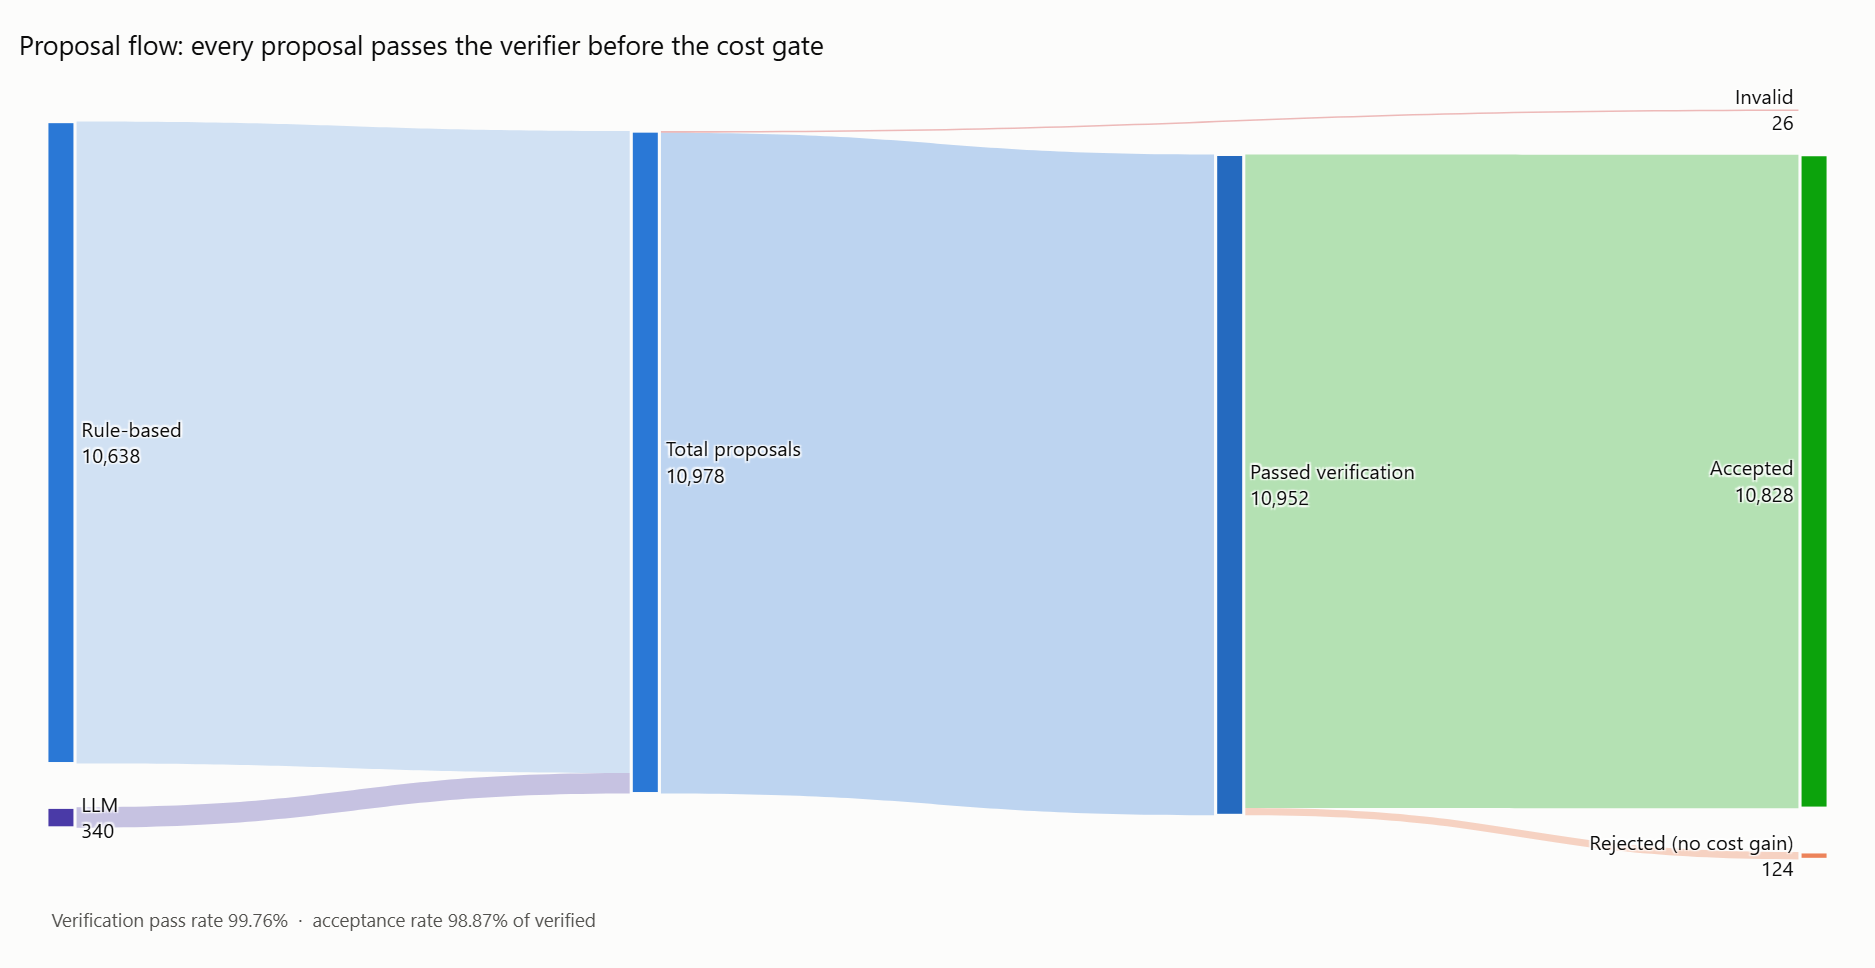
\includegraphics[width=\textwidth]{report_figures/sankey_gemini.png}
\caption{Sankey diagram showing the flow of 10,978 proposals from submission through verification to the accept/reject decision. The 26 invalid proposals are visible as a narrow band}
\label{fig:sankey}
\end{figure}

\subsection{Grouped Bar Chart: Outcomes by Optimization Type}

\begin{figure}[H]
\centering
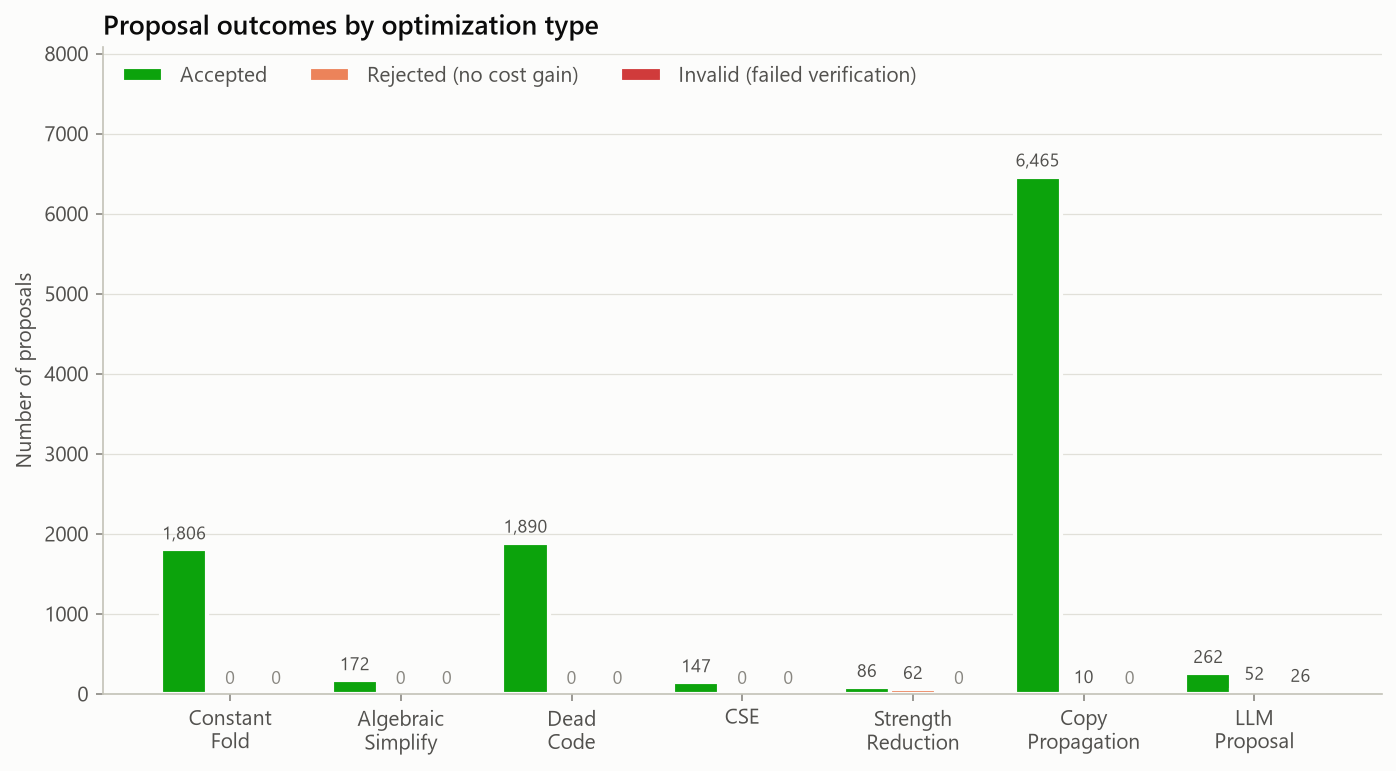
\includegraphics[width=\textwidth]{report_figures/outcomes_by_type_gemini.png}
\caption{Accept, reject, and invalid counts for each optimization type. Copy propagation accounts for the most accepted changes}
\label{fig:outcomes}
\end{figure}

\subsection{Line Chart: Cost Trajectory over Iterations}

\begin{figure}[H]
\centering
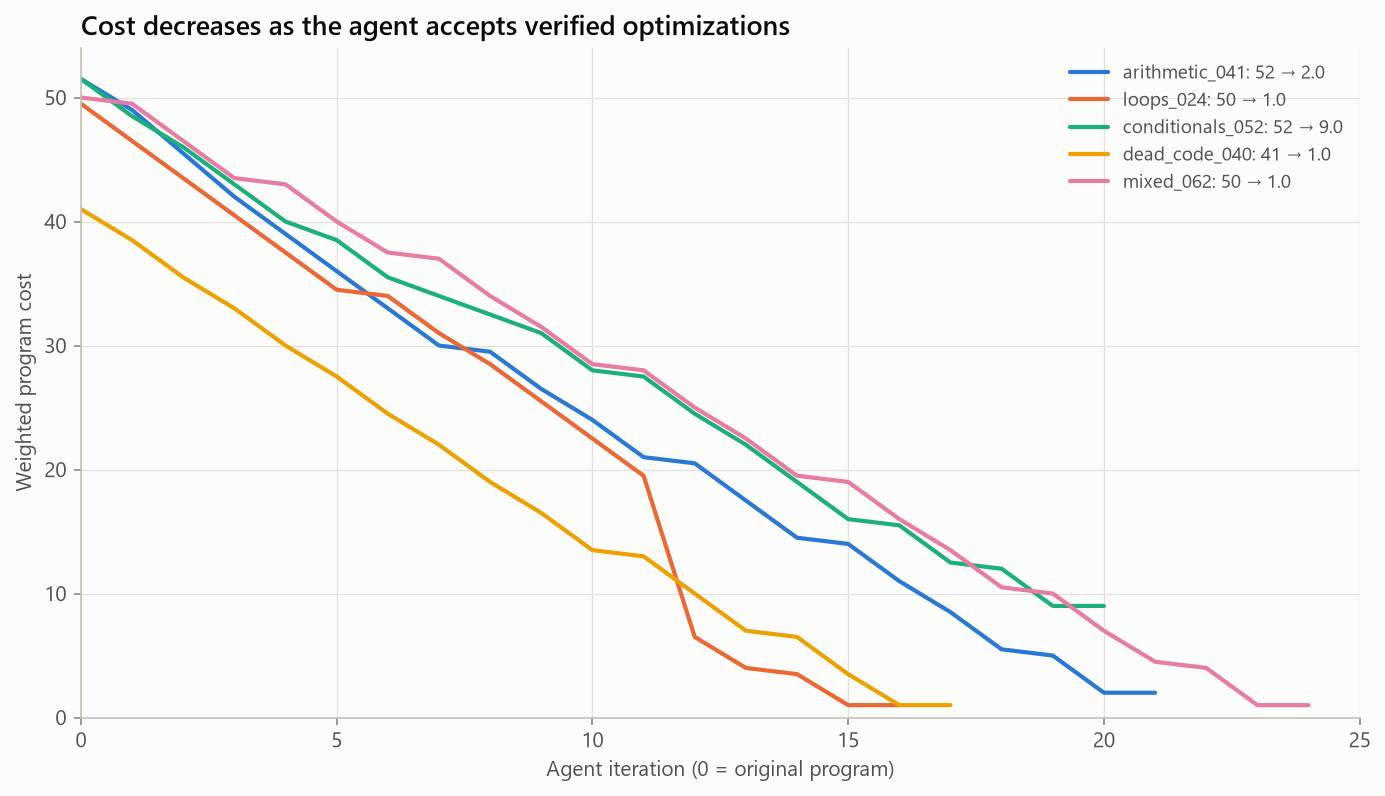
\includegraphics[width=\textwidth]{report_figures/cost_over_iterations_gemini.png}
\caption{Weighted cost at each iteration for five representative programs. Cost decreases rapidly during early iterations and levels off as optimization converges}
\label{fig:trajectory}
\end{figure}

\subsection{Pie Chart: Accepted Optimization Types}

\begin{figure}[H]
\centering
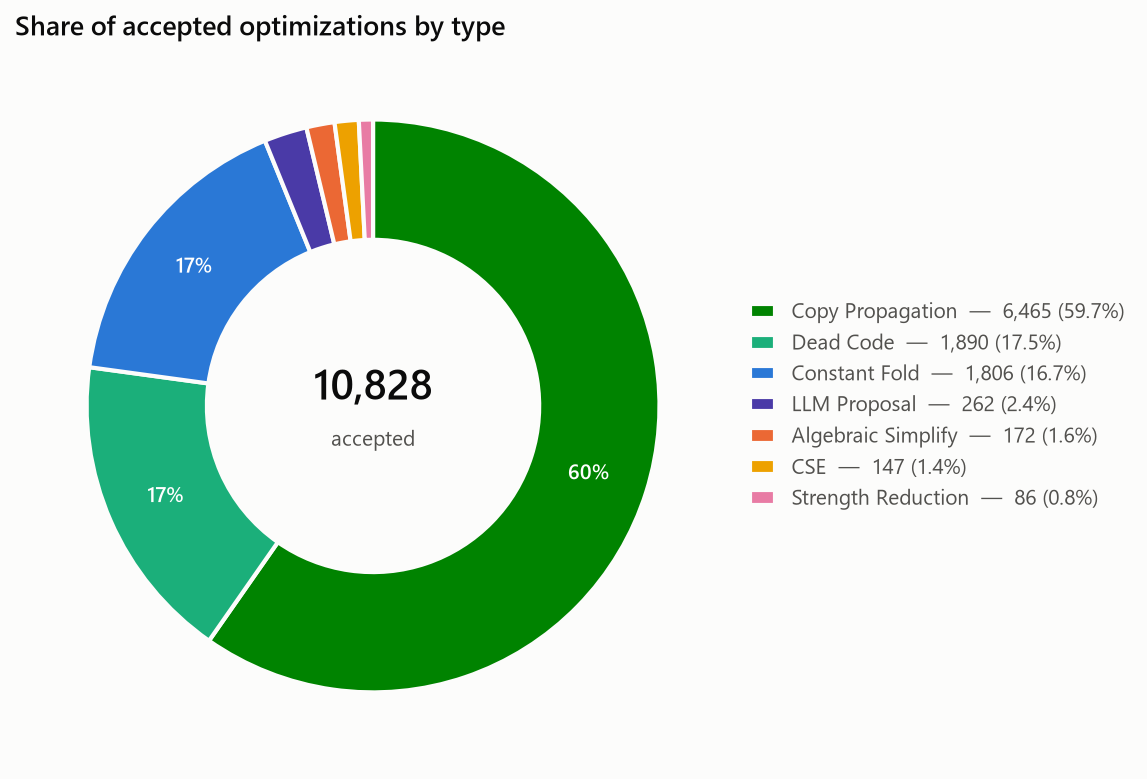
\includegraphics[width=0.9\textwidth]{report_figures/accepted_types_gemini.png}
\caption{Breakdown of accepted optimizations by optimization type. Copy propagation accounts for the largest share of accepted changes}
\label{fig:pie}
\end{figure}

\subsection{Scatter Plot: Steps vs.\ Cost Improvement}

\begin{figure}[H]
\centering
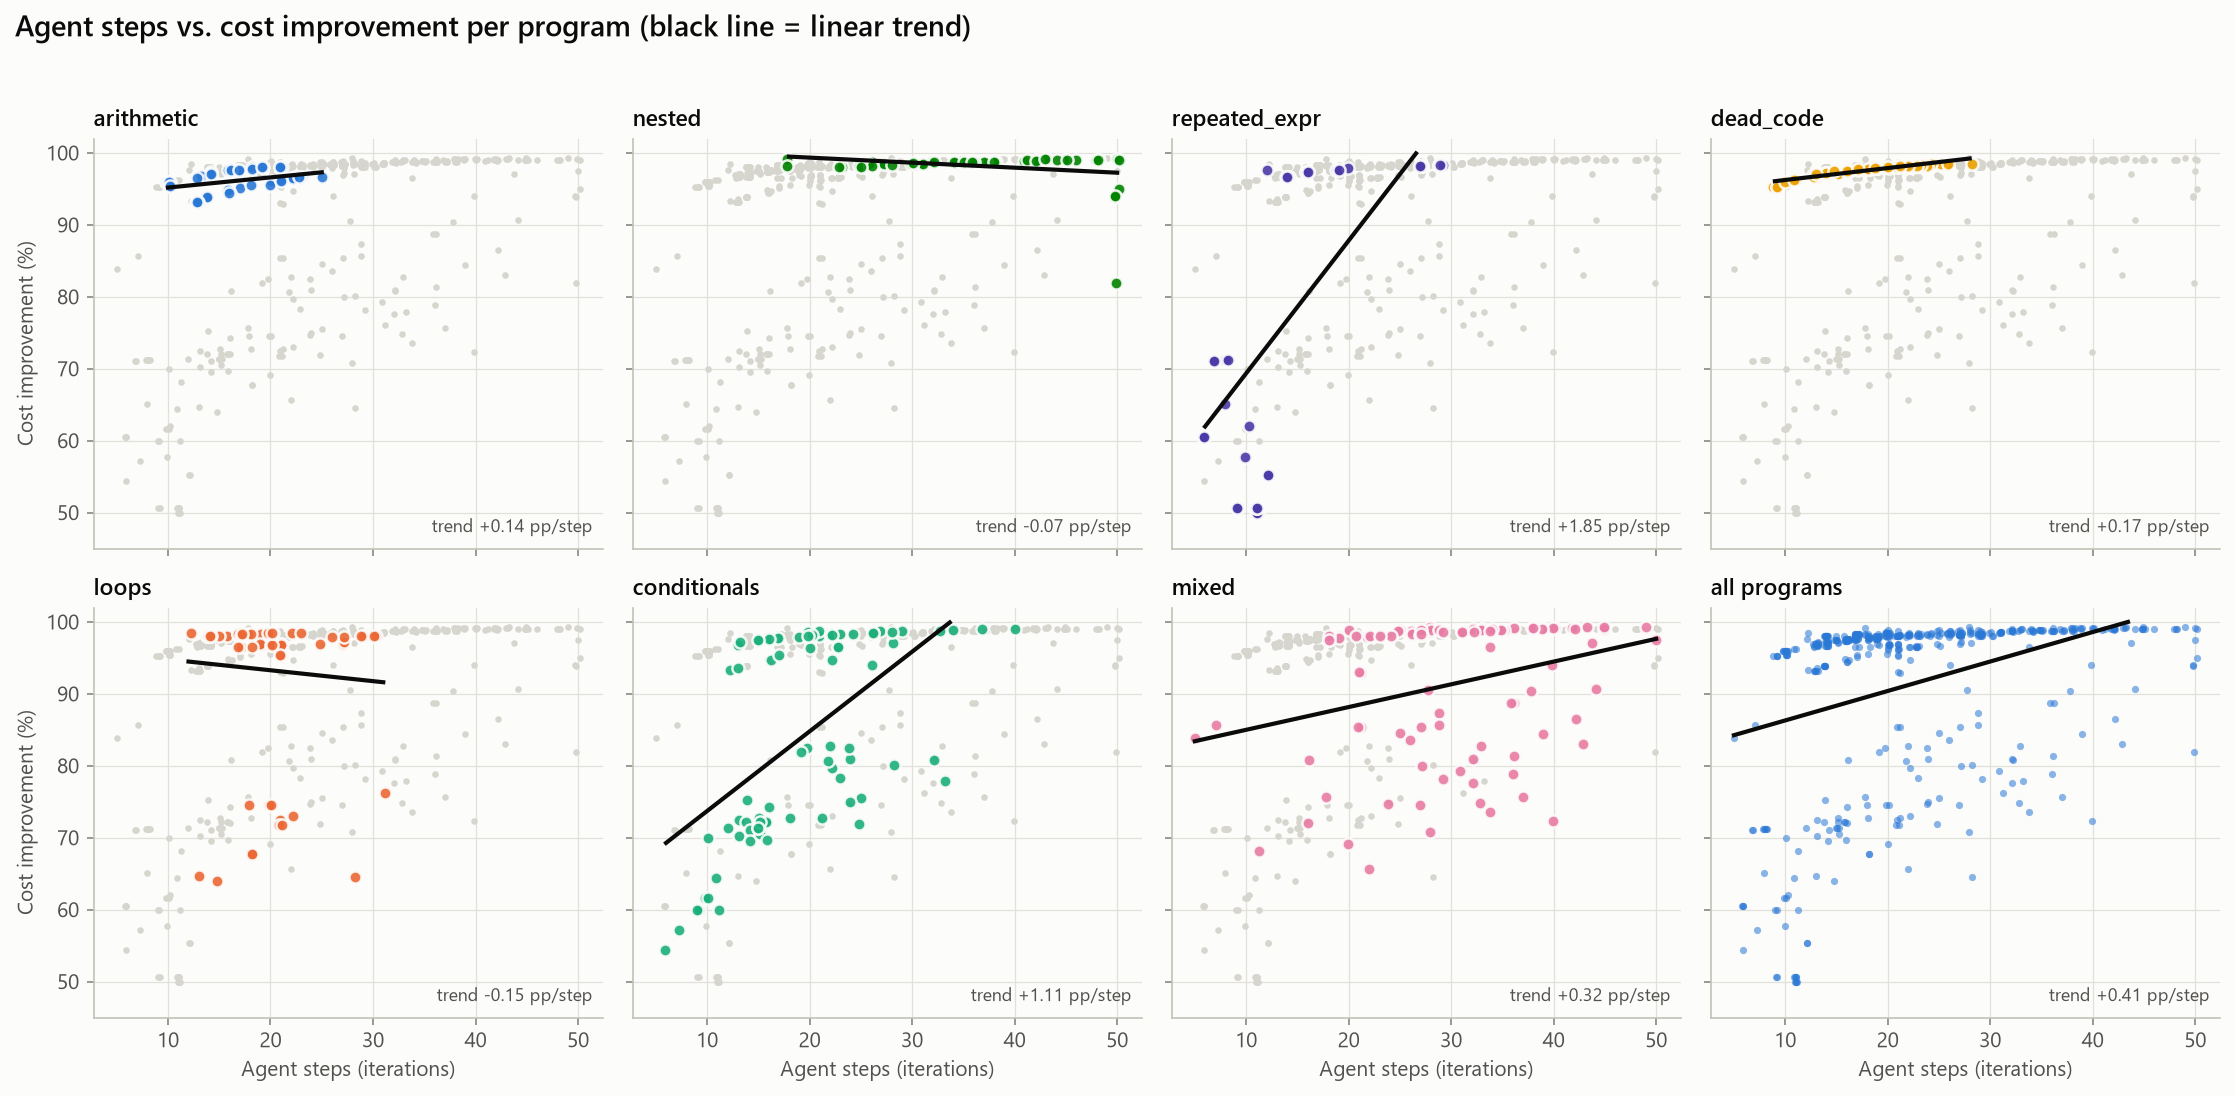
\includegraphics[width=\textwidth]{report_figures/steps_vs_improvement_gemini.png}
\caption{Agent steps versus percentage cost improvement across the program categories}
\label{fig:scatter}
\end{figure}

\subsection{Heatmap: Category vs.\ Optimization Type}

\begin{figure}[H]
\centering
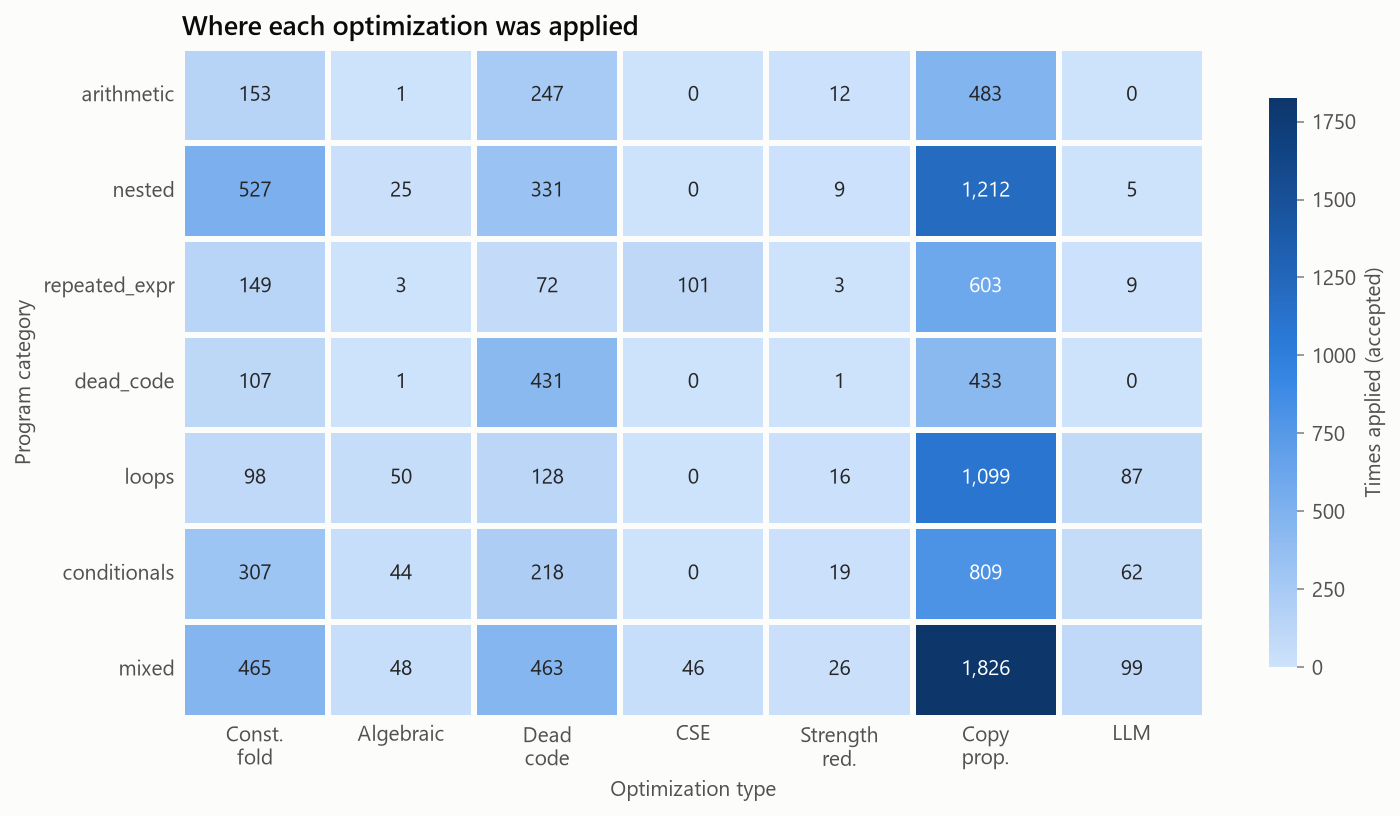
\includegraphics[width=\textwidth]{report_figures/heatmap_gemini.png}
\caption{Number of accepted optimizations for each program category and optimization type}
\label{fig:heatmap}
\end{figure}

\subsection{Comparison Charts: Rule-Only vs.\ Rule + LLM}

\begin{figure}[H]
\centering
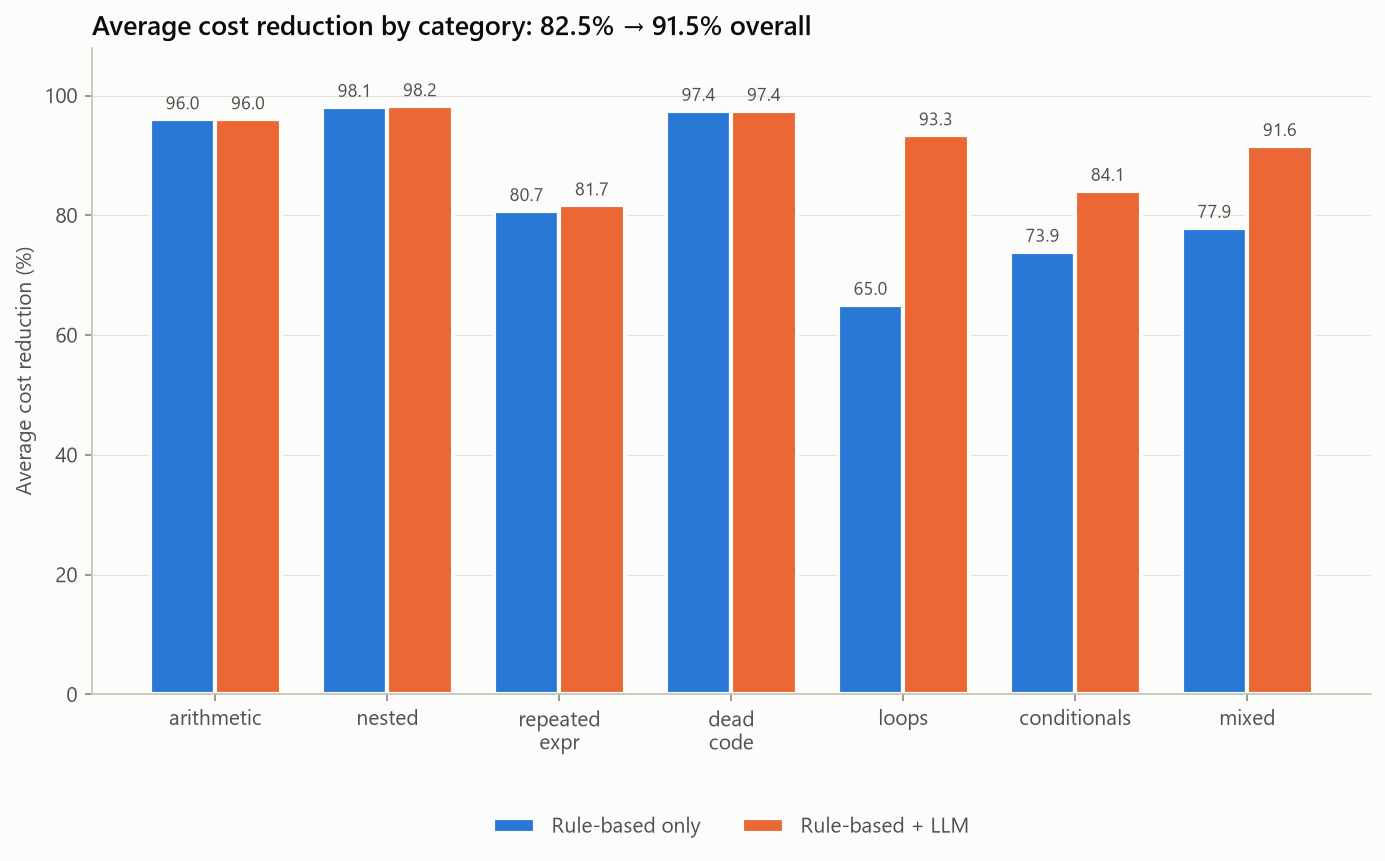
\includegraphics[width=0.9\textwidth]{report_figures/comparison_gemini.png}
\caption{Average cost reduction per category comparing rule-only optimization with rule + Gemini. Loops rise from 65\% to 93\%}
\label{fig:cmp-gemini}
\end{figure}

\begin{figure}[H]
\centering
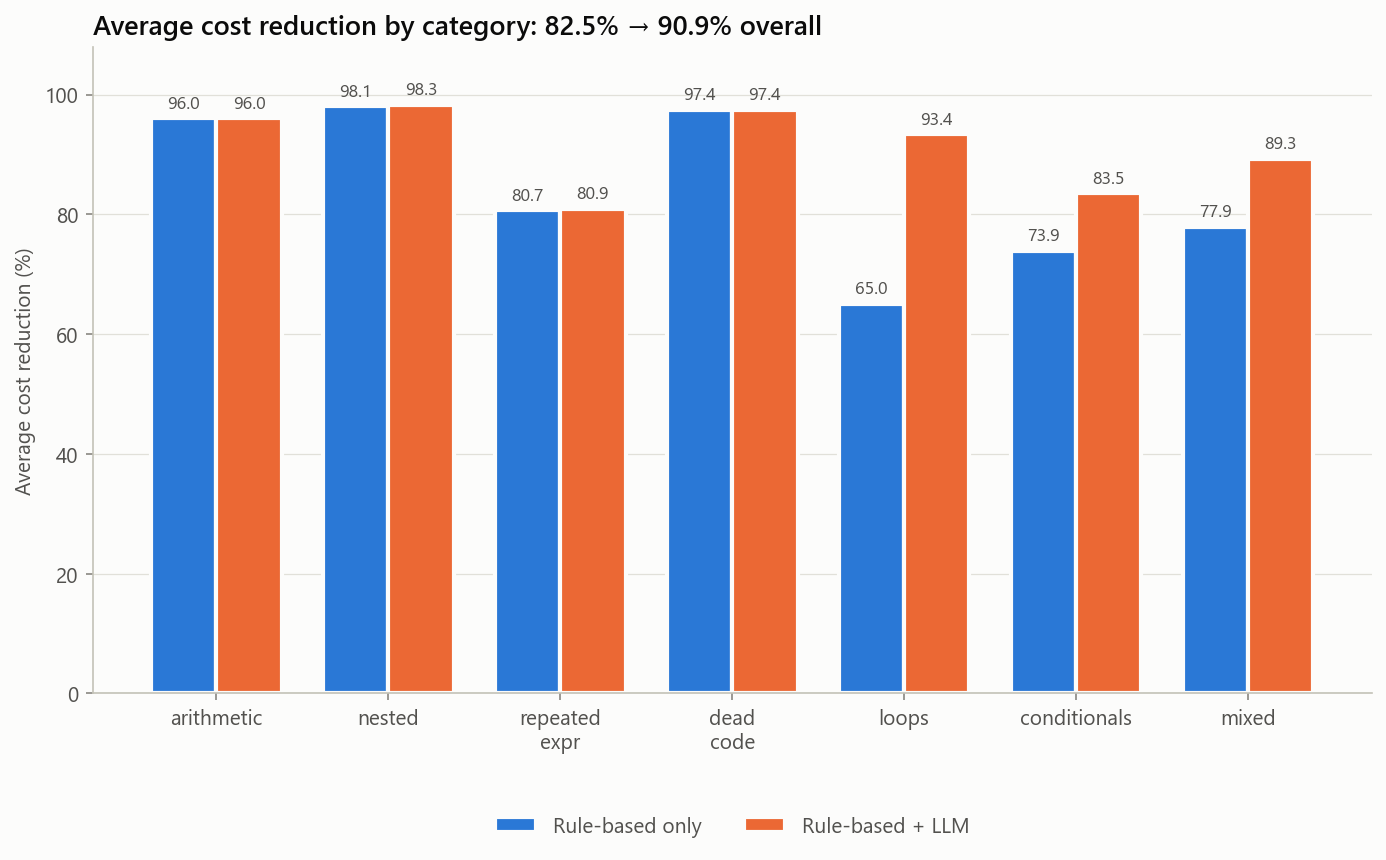
\includegraphics[width=0.9\textwidth]{report_figures/comparison_groq.png}
\caption{Rule-only against rule + Groq. The pattern is the same as with Gemini}
\label{fig:cmp-groq}
\end{figure}

\begin{figure}[H]
\centering
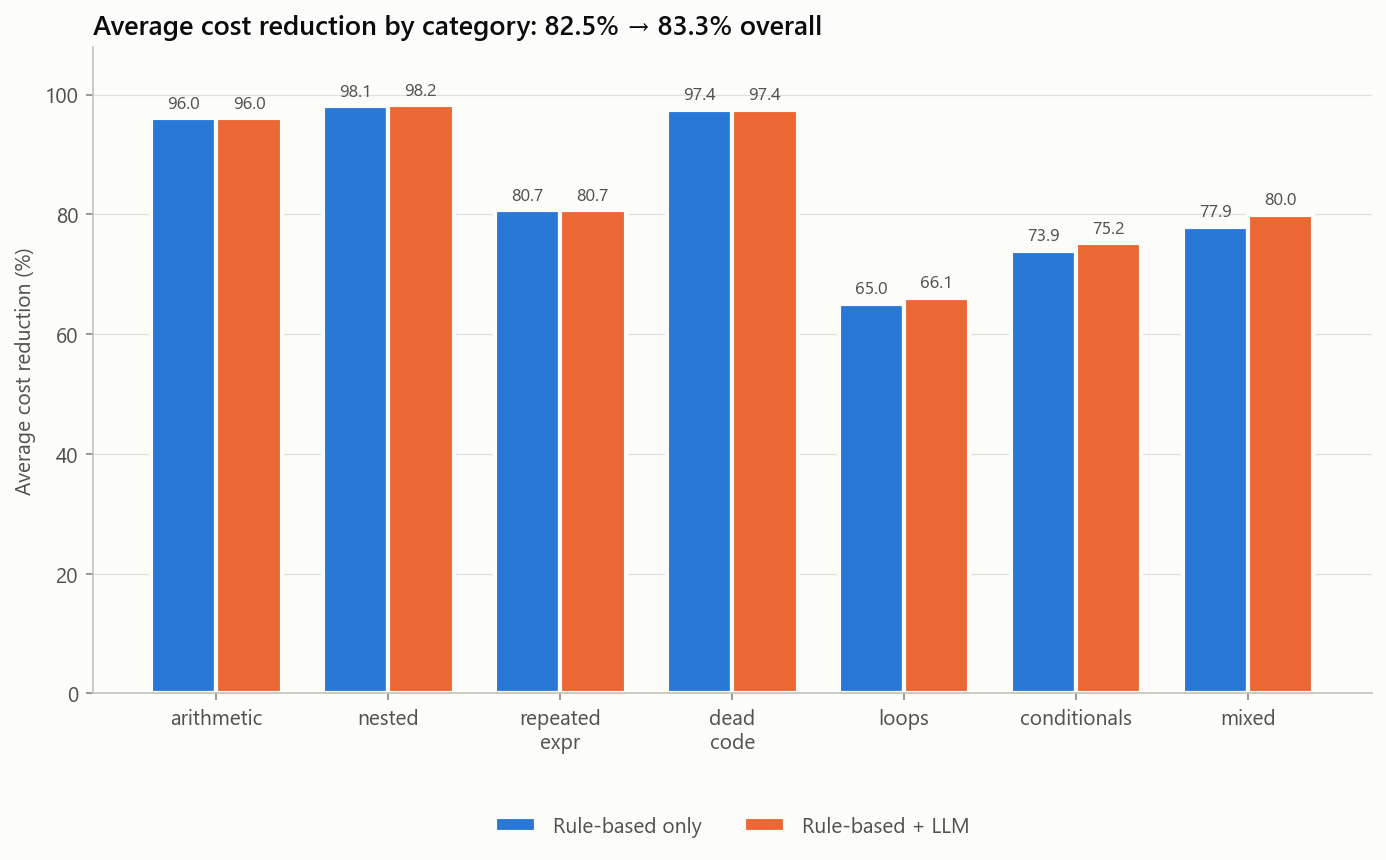
\includegraphics[width=0.9\textwidth]{report_figures/comparison_ollama.png}
\caption{Rule-only against rule + the local Ollama model. The gains are small but come with no internet connection}
\label{fig:cmp-ollama}
\end{figure}

\subsection{Analysis Charts for the Groq Run}

Figures~\ref{fig:sankey-groq} to \ref{fig:heatmap-groq} repeat the six charts for the run with Groq. The picture is close to the Gemini run: the same optimization types dominate, and only 6 proposals fail verification.

\begin{figure}[H]
\centering
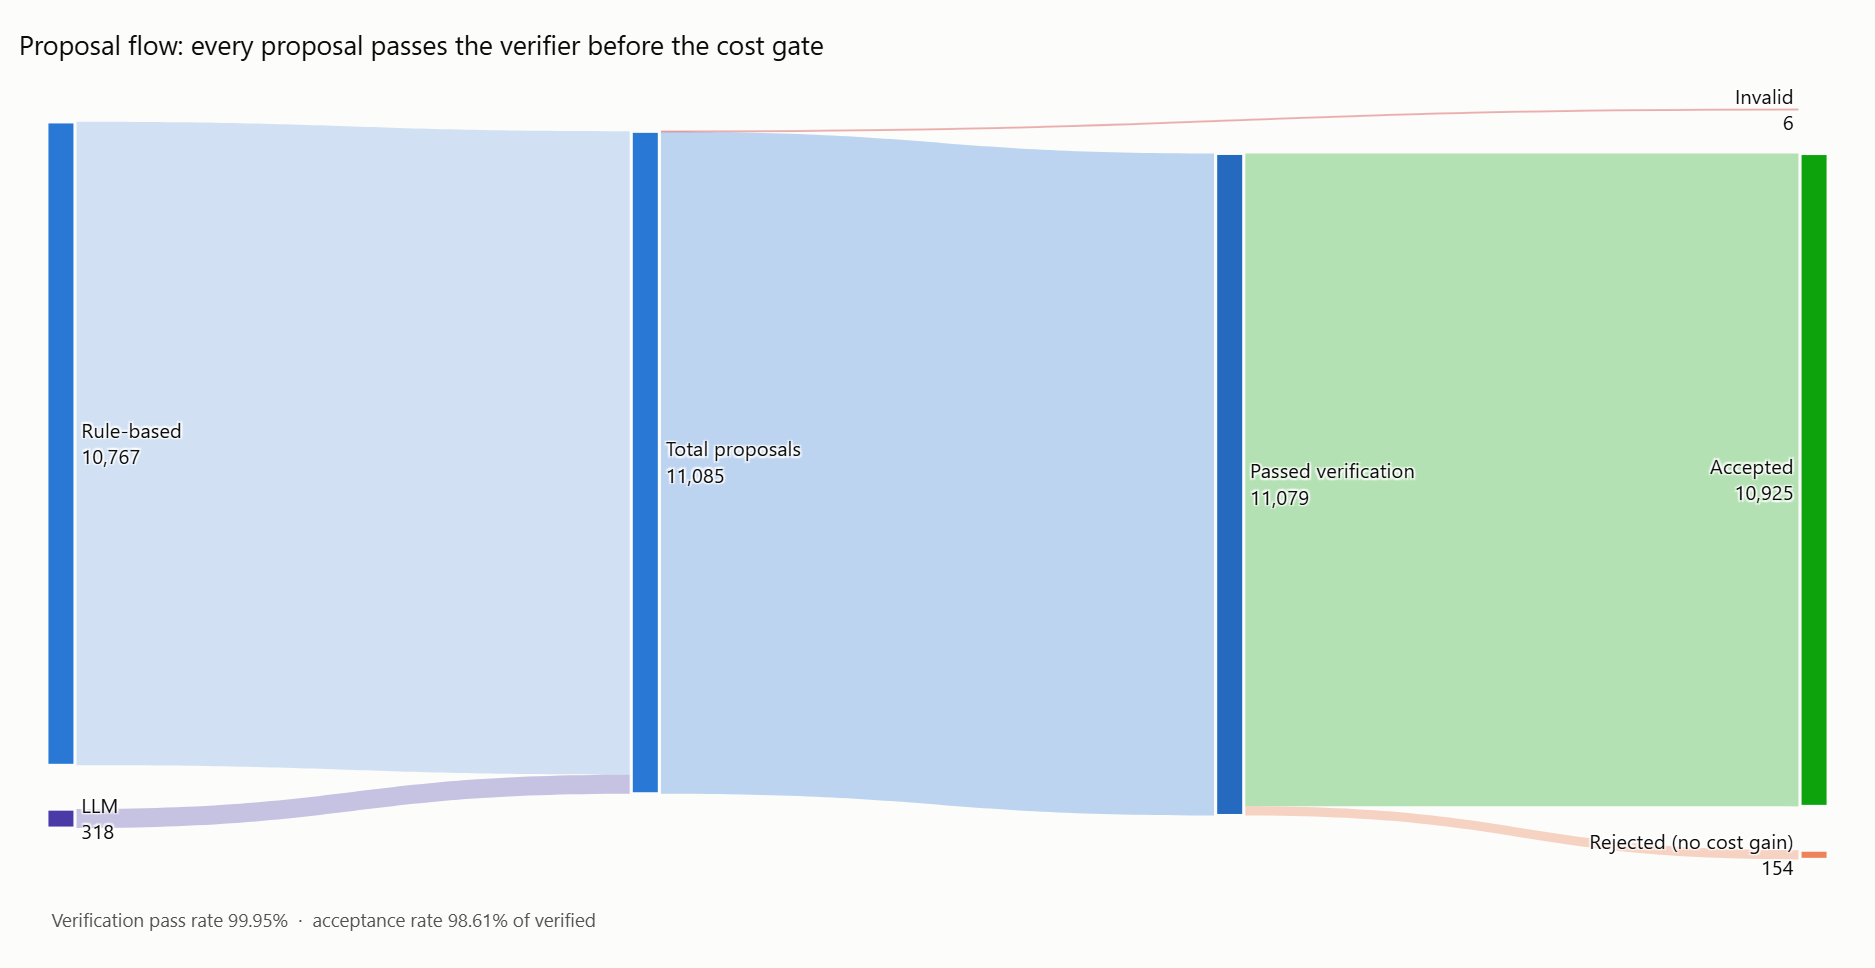
\includegraphics[width=\textwidth]{report_figures/sankey_groq.png}
\caption{Groq run: flow of the 11,085 proposals. Only 6 LLM proposals were invalid, so the band of blocked proposals is barely visible}
\label{fig:sankey-groq}
\end{figure}

\begin{figure}[H]
\centering
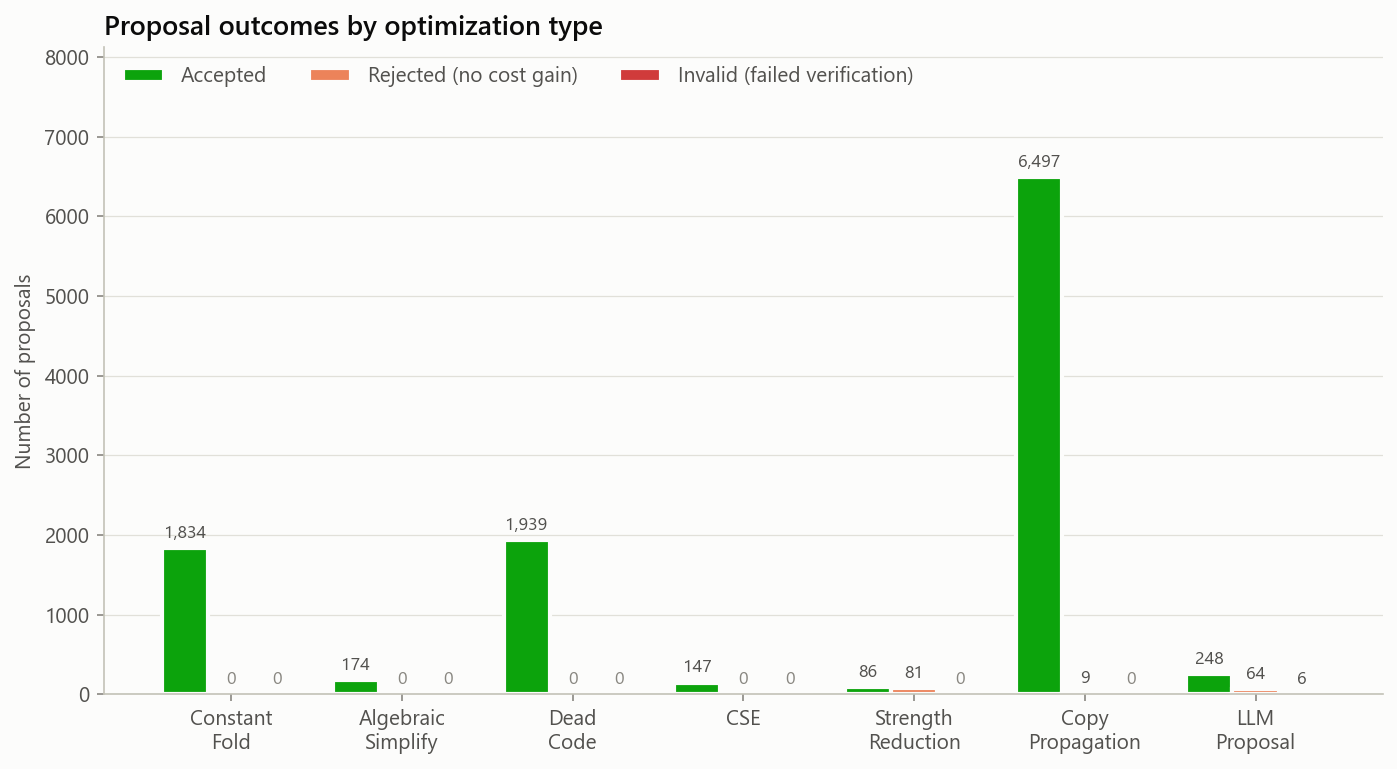
\includegraphics[width=\textwidth]{report_figures/outcomes_by_type_groq.png}
\caption{Groq run: accept, reject, and invalid counts for each optimization type}
\label{fig:outcomes-groq}
\end{figure}

\begin{figure}[H]
\centering
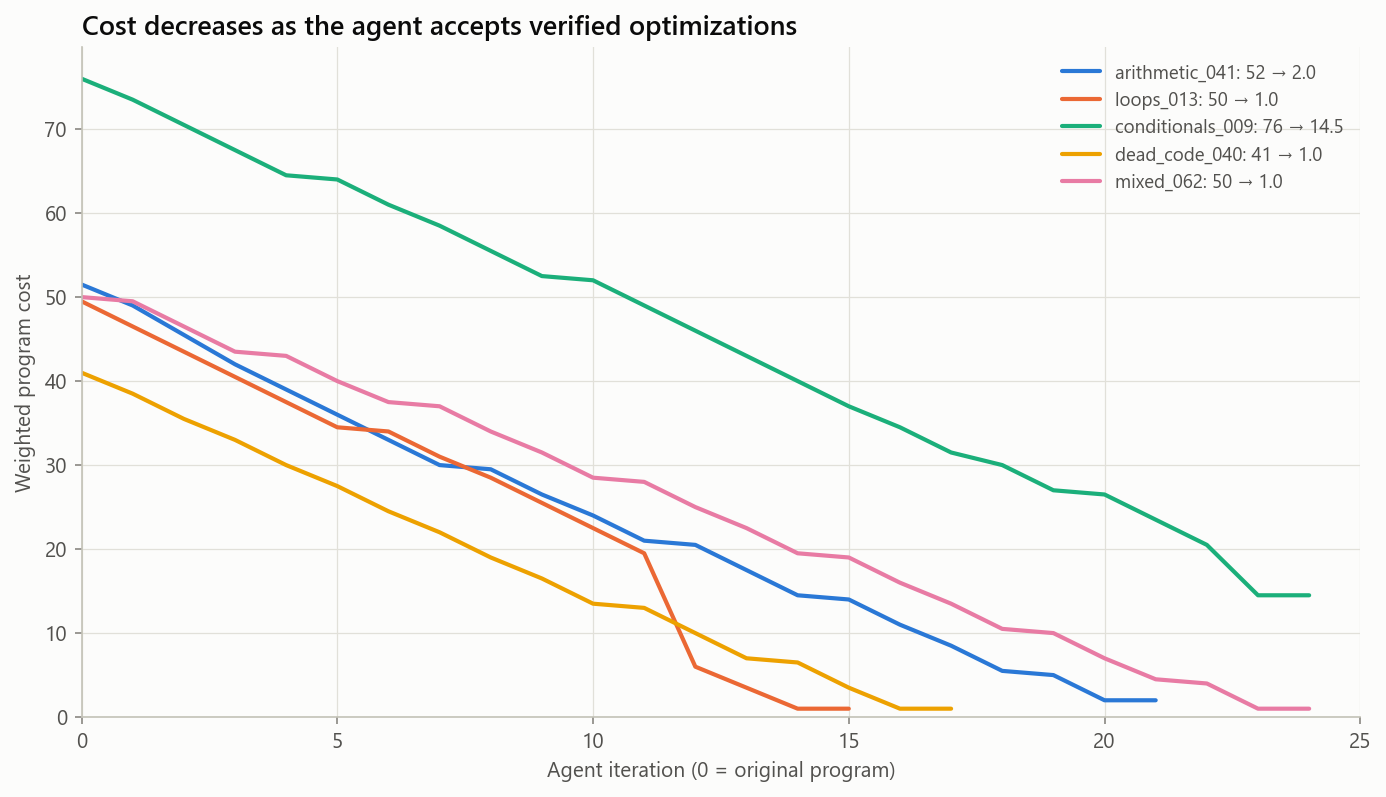
\includegraphics[width=\textwidth]{report_figures/cost_over_iterations_groq.png}
\caption{Groq run: weighted cost at each iteration for five representative programs}
\label{fig:trajectory-groq}
\end{figure}

\begin{figure}[H]
\centering
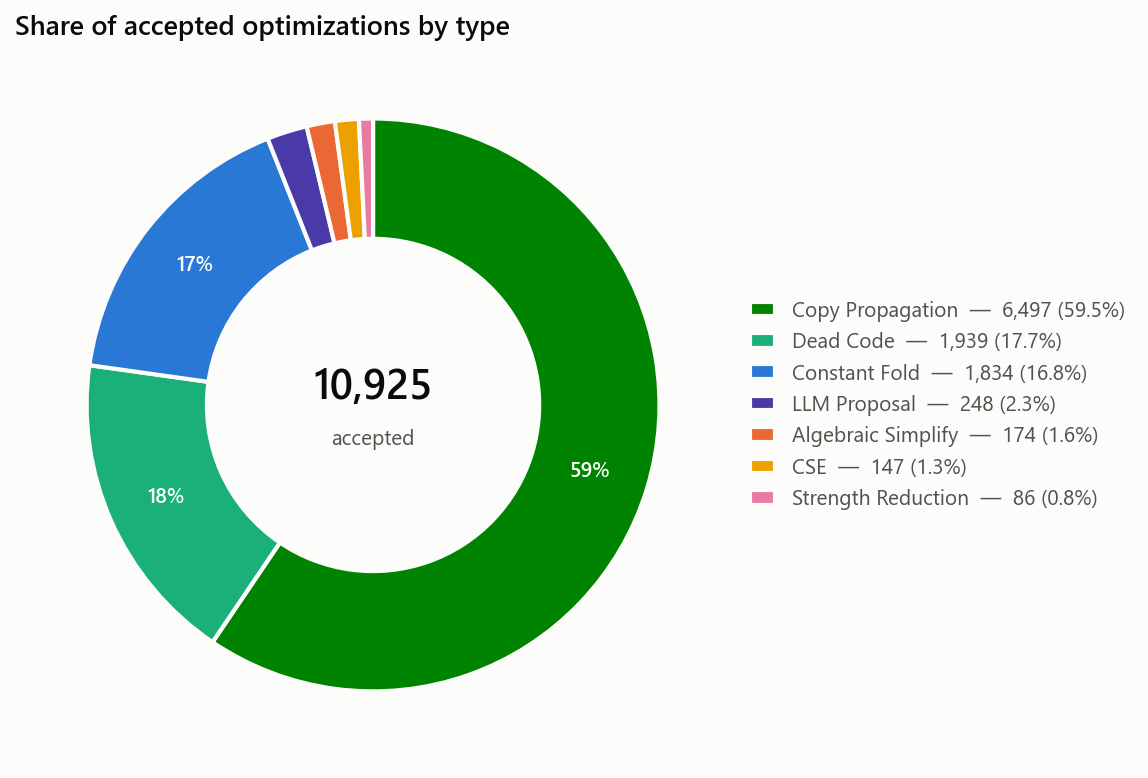
\includegraphics[width=0.9\textwidth]{report_figures/accepted_types_groq.png}
\caption{Groq run: breakdown of accepted optimizations by type}
\label{fig:pie-groq}
\end{figure}

\begin{figure}[H]
\centering
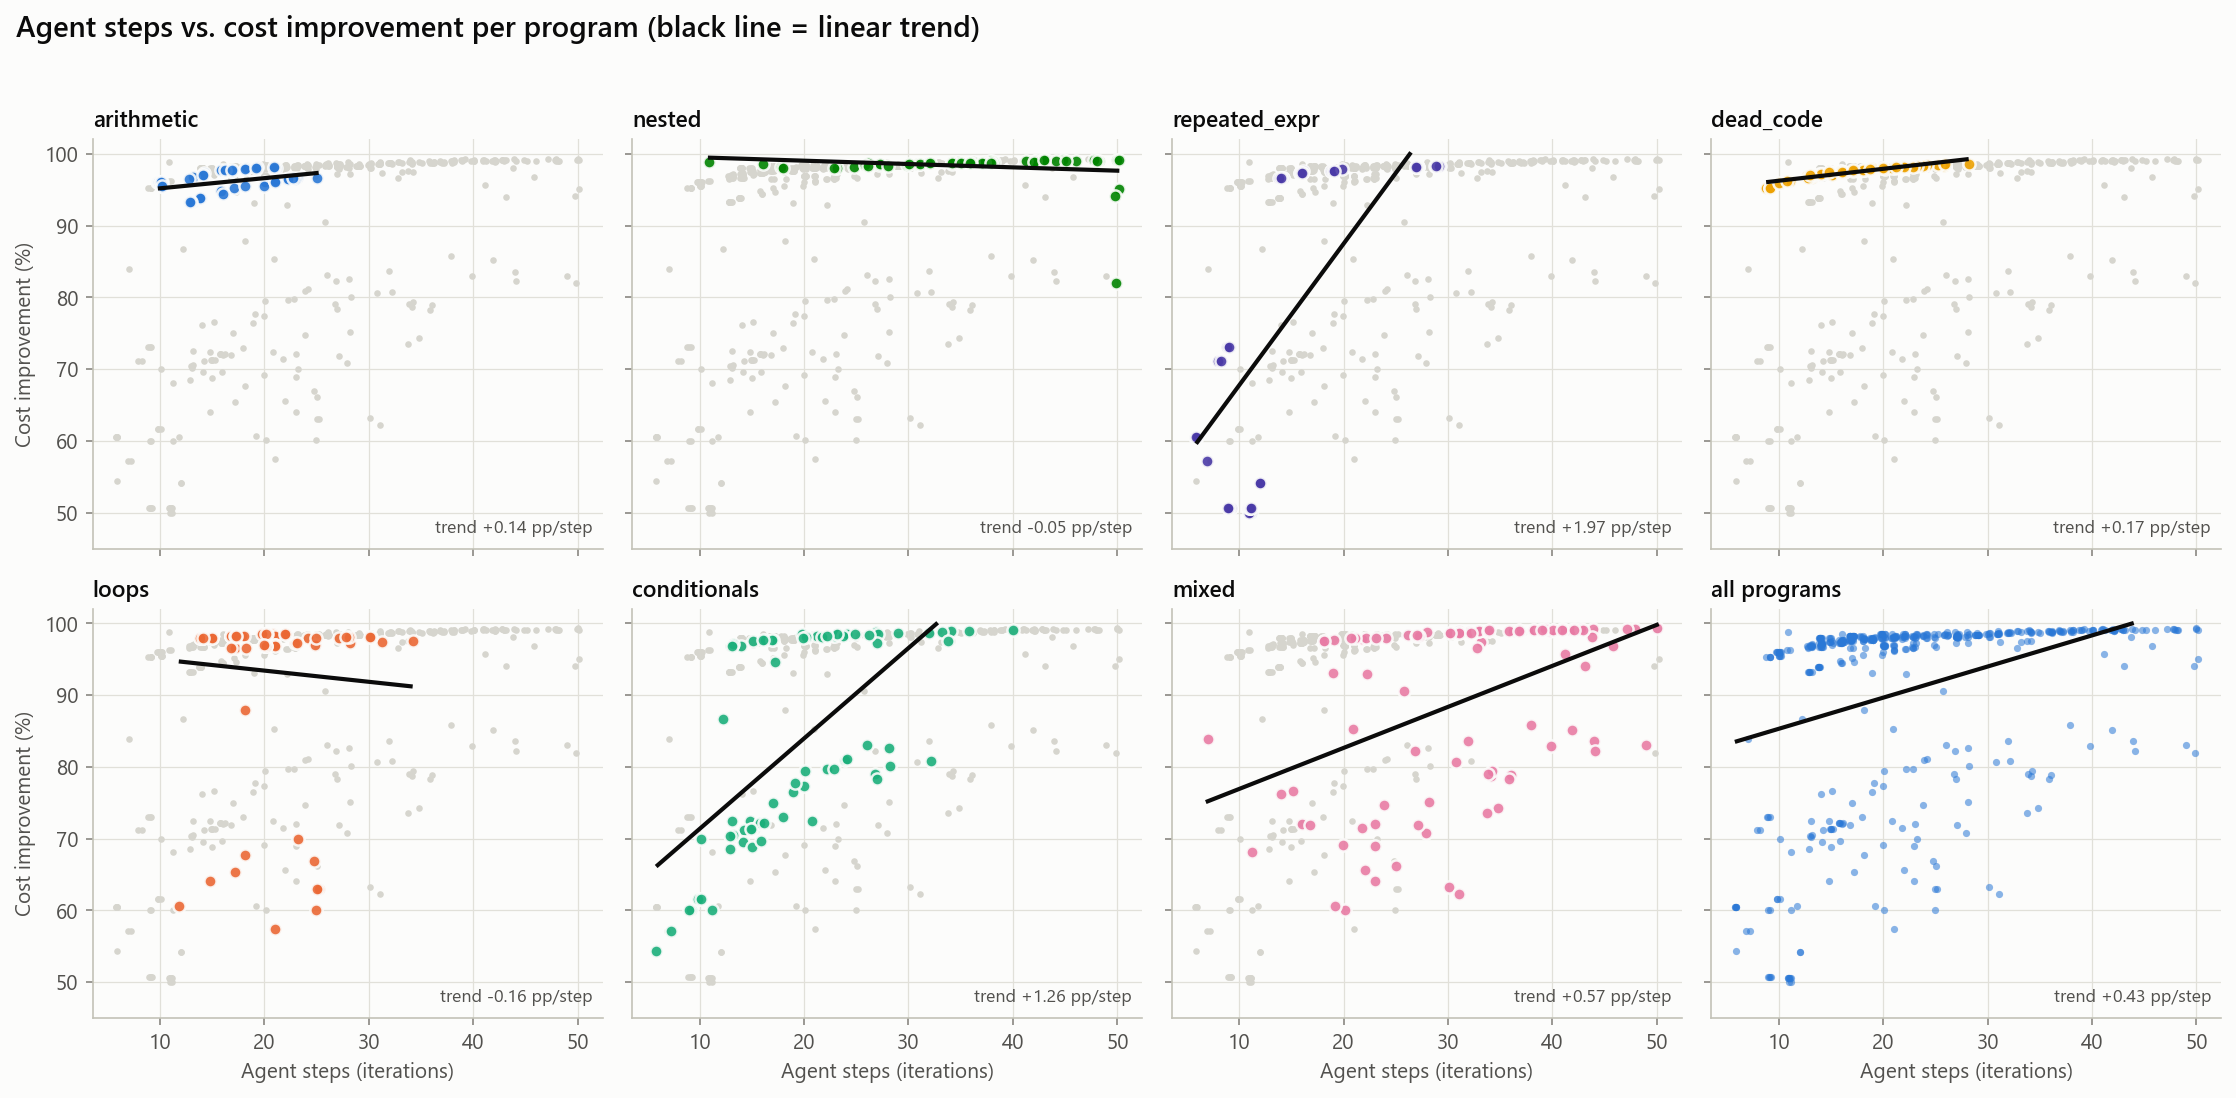
\includegraphics[width=\textwidth]{report_figures/steps_vs_improvement_groq.png}
\caption{Groq run: agent steps versus percentage cost improvement}
\label{fig:scatter-groq}
\end{figure}

\begin{figure}[H]
\centering
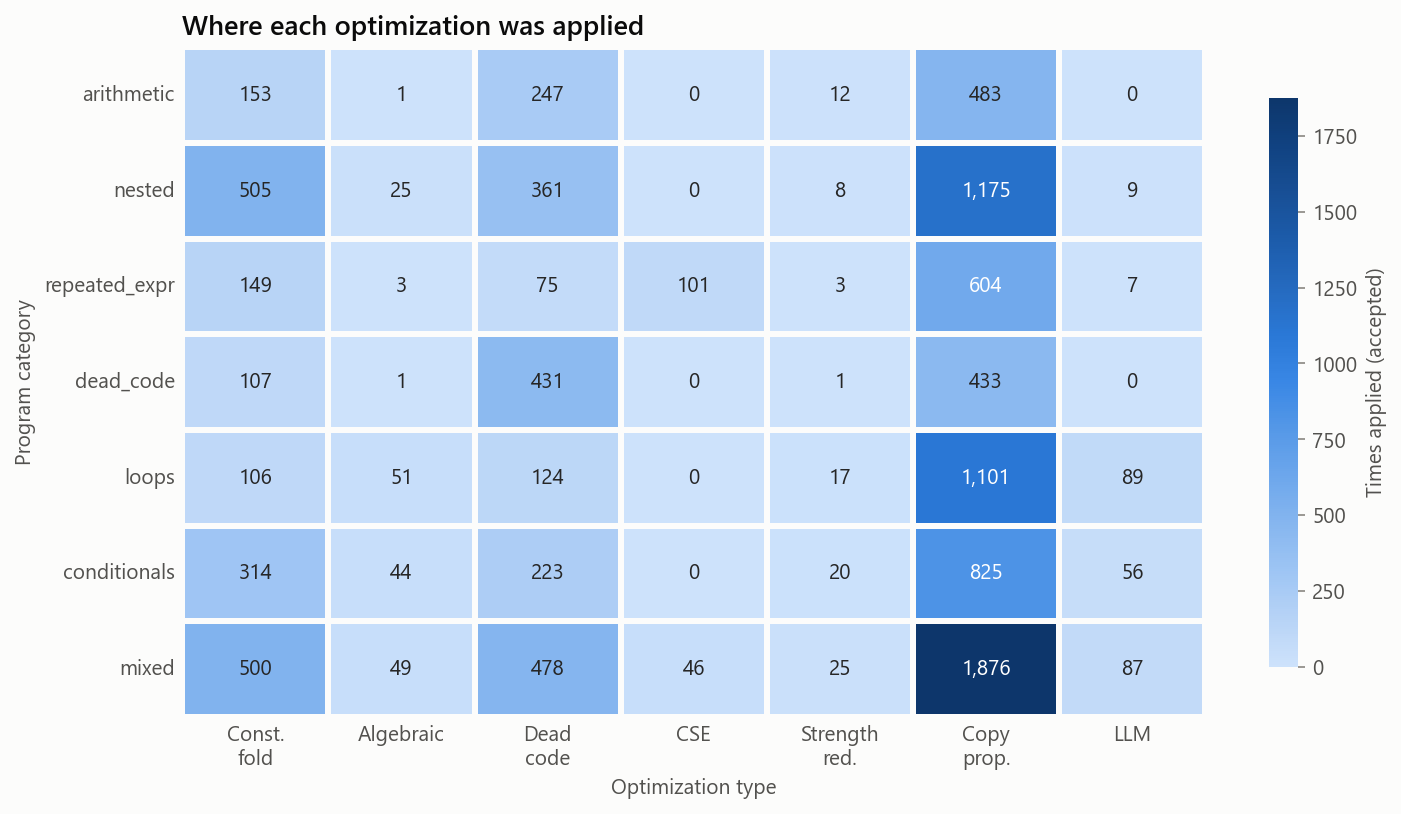
\includegraphics[width=\textwidth]{report_figures/heatmap_groq.png}
\caption{Groq run: accepted optimizations for each program category and optimization type}
\label{fig:heatmap-groq}
\end{figure}

\subsection{Analysis Charts for the Ollama Run}

Figures~\ref{fig:sankey-ollama} to \ref{fig:heatmap-ollama} show the same charts for the offline run with the local model. Here the band of invalid proposals is clearly visible: 113 of the local model's proposals were wrong, and every one was blocked by the verifier.

\begin{figure}[H]
\centering
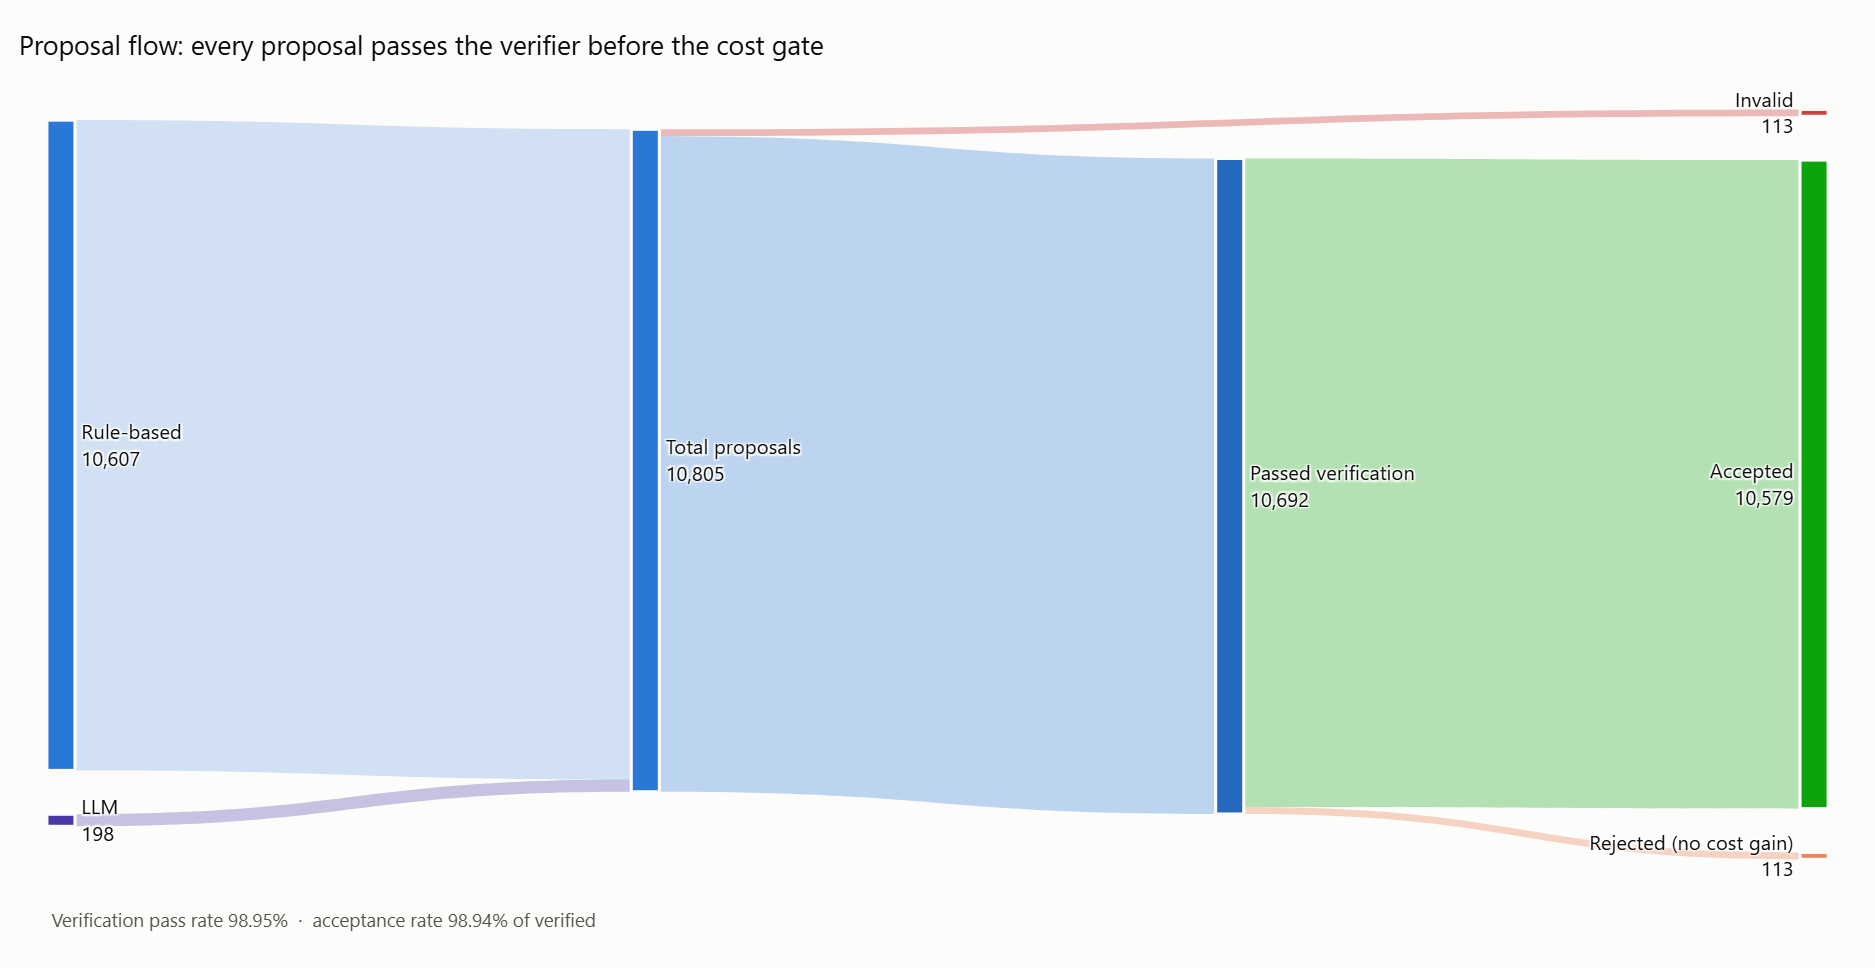
\includegraphics[width=\textwidth]{report_figures/sankey_ollama.png}
\caption{Ollama run: flow of the 10,805 proposals. The 113 invalid LLM proposals form a visible band that ends at the verifier}
\label{fig:sankey-ollama}
\end{figure}

\begin{figure}[H]
\centering
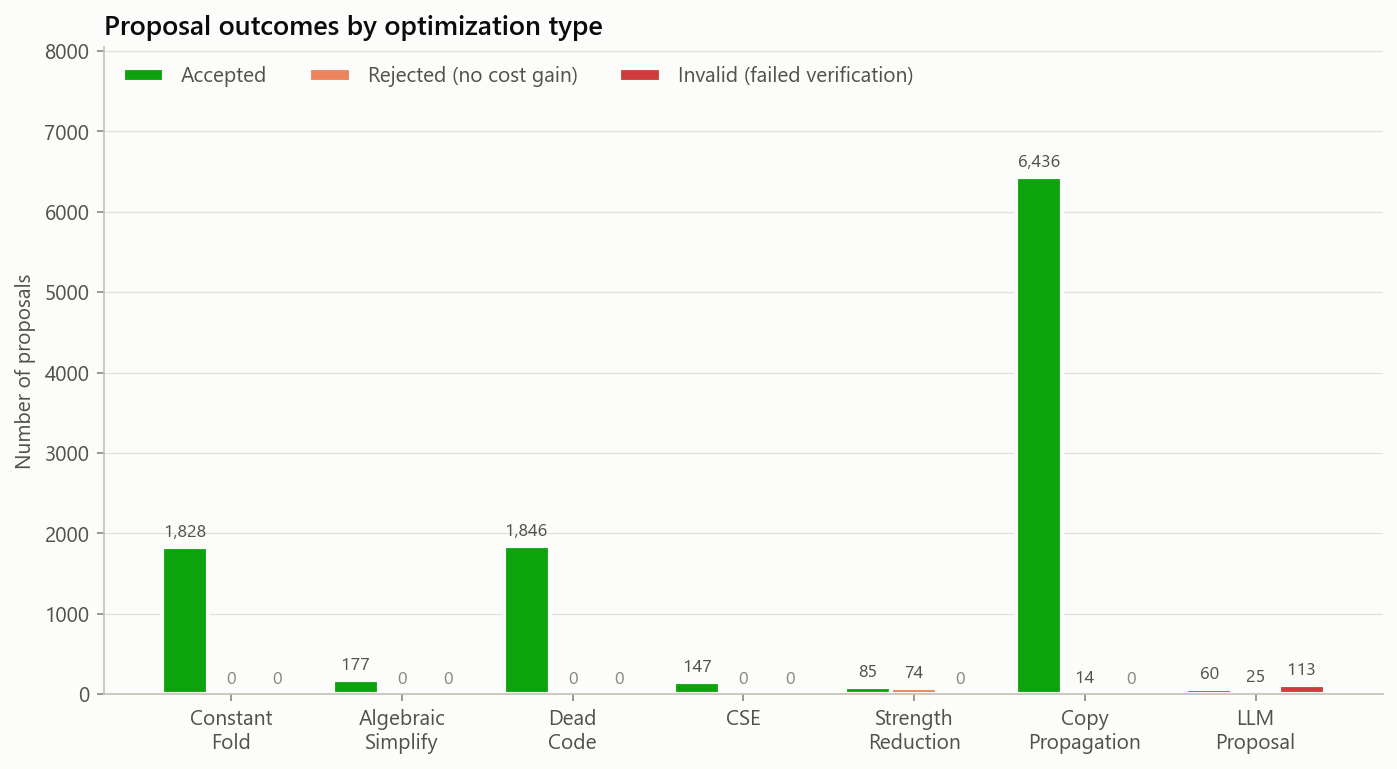
\includegraphics[width=\textwidth]{report_figures/outcomes_by_type_ollama.png}
\caption{Ollama run: accept, reject, and invalid counts for each optimization type. The invalid bar belongs to the LLM proposals}
\label{fig:outcomes-ollama}
\end{figure}

\begin{figure}[H]
\centering
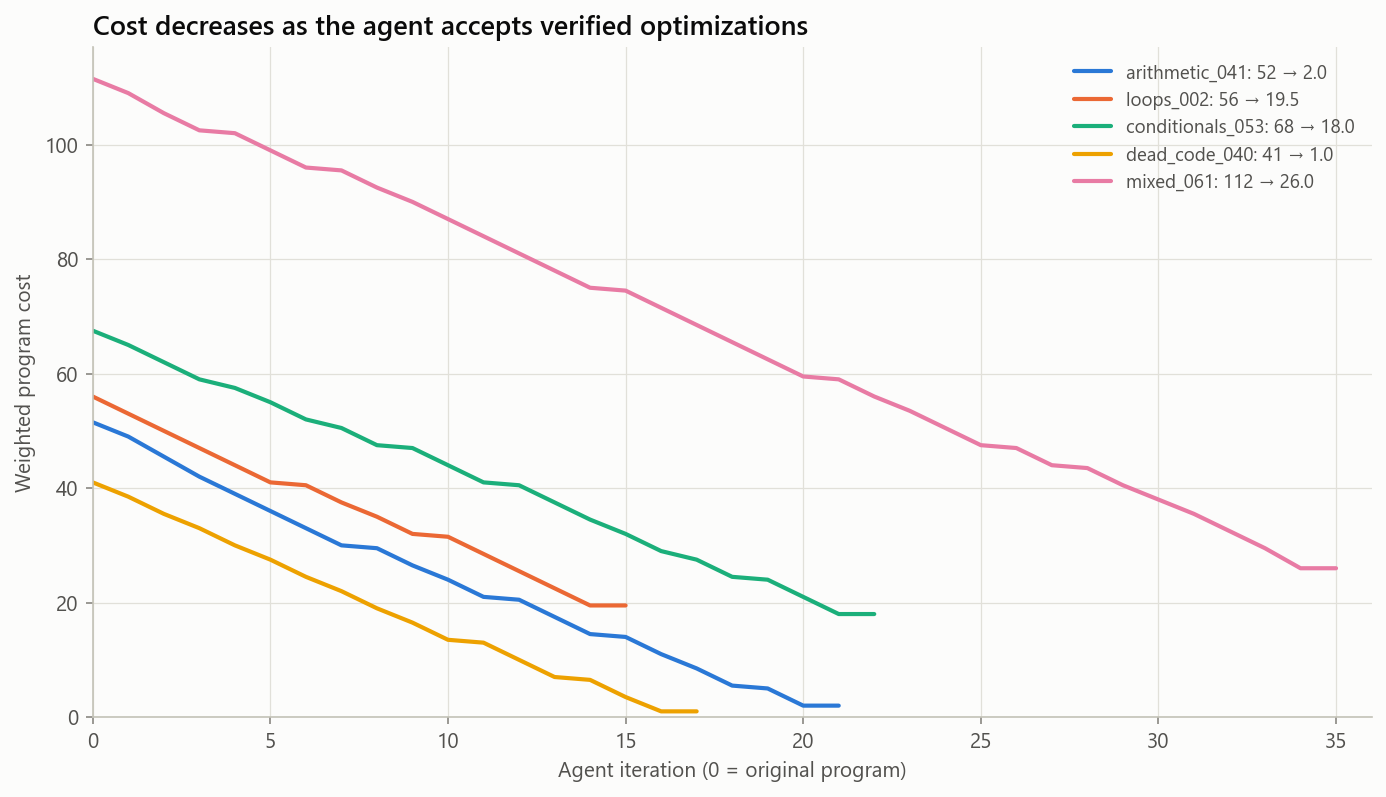
\includegraphics[width=\textwidth]{report_figures/cost_over_iterations_ollama.png}
\caption{Ollama run: weighted cost at each iteration for five representative programs}
\label{fig:trajectory-ollama}
\end{figure}

\begin{figure}[H]
\centering
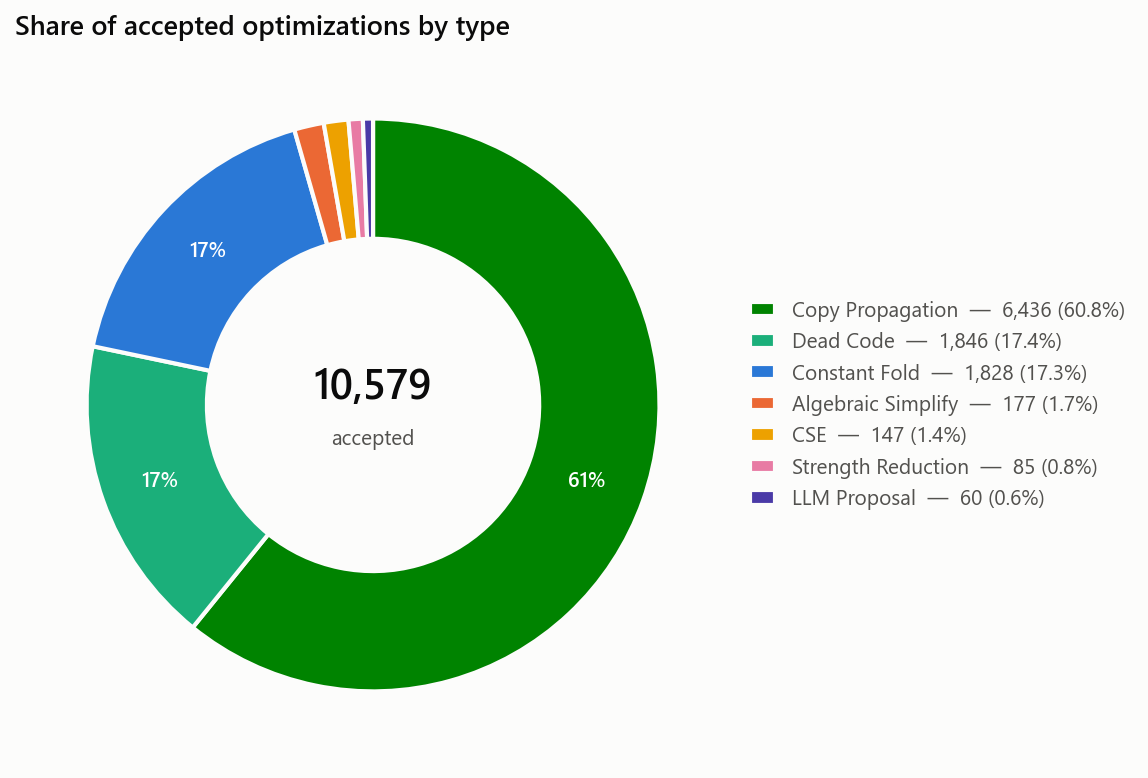
\includegraphics[width=0.9\textwidth]{report_figures/accepted_types_ollama.png}
\caption{Ollama run: breakdown of accepted optimizations by type}
\label{fig:pie-ollama}
\end{figure}

\begin{figure}[H]
\centering
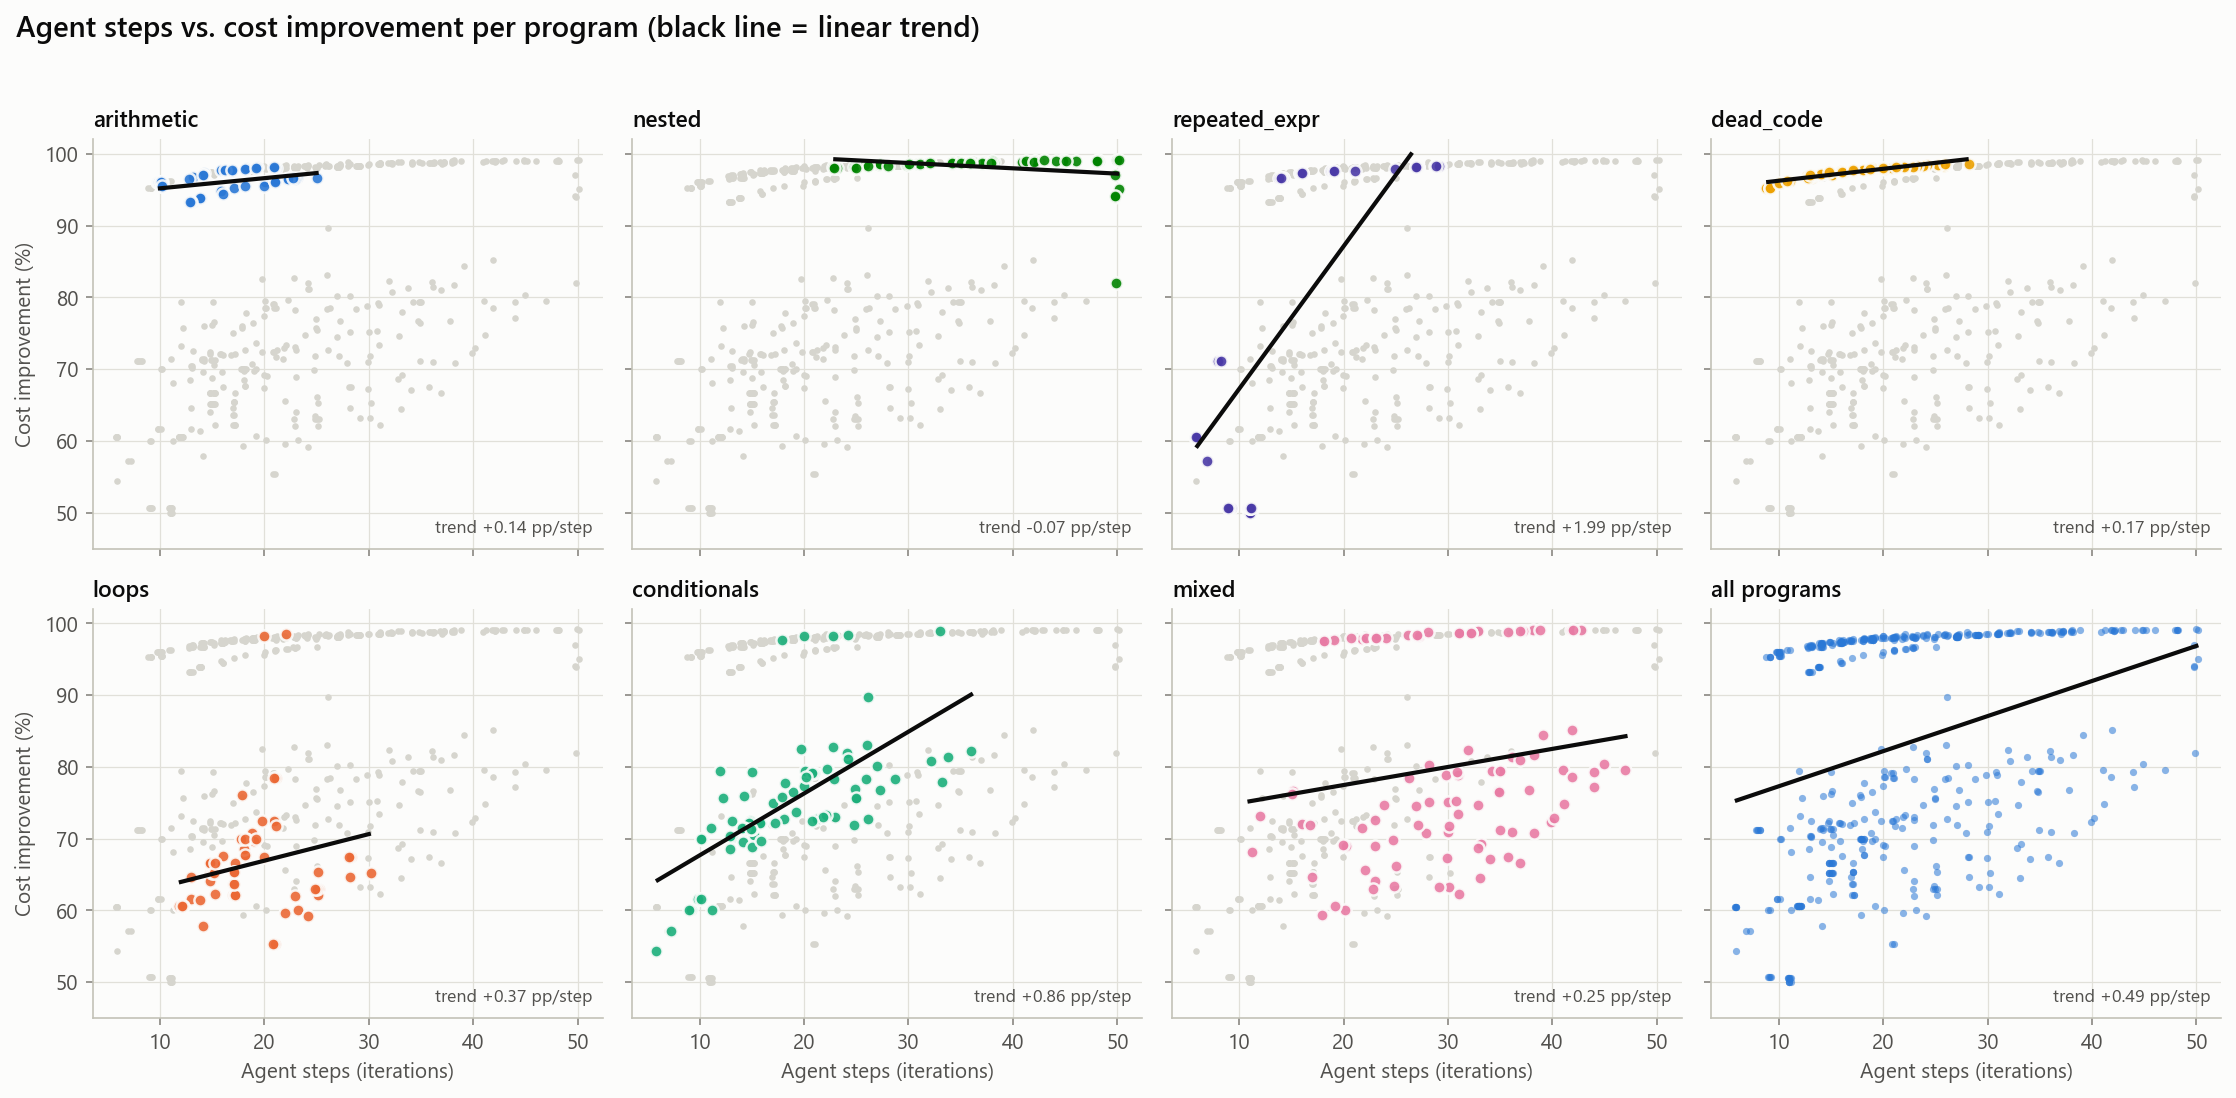
\includegraphics[width=\textwidth]{report_figures/steps_vs_improvement_ollama.png}
\caption{Ollama run: agent steps versus percentage cost improvement}
\label{fig:scatter-ollama}
\end{figure}

\begin{figure}[H]
\centering
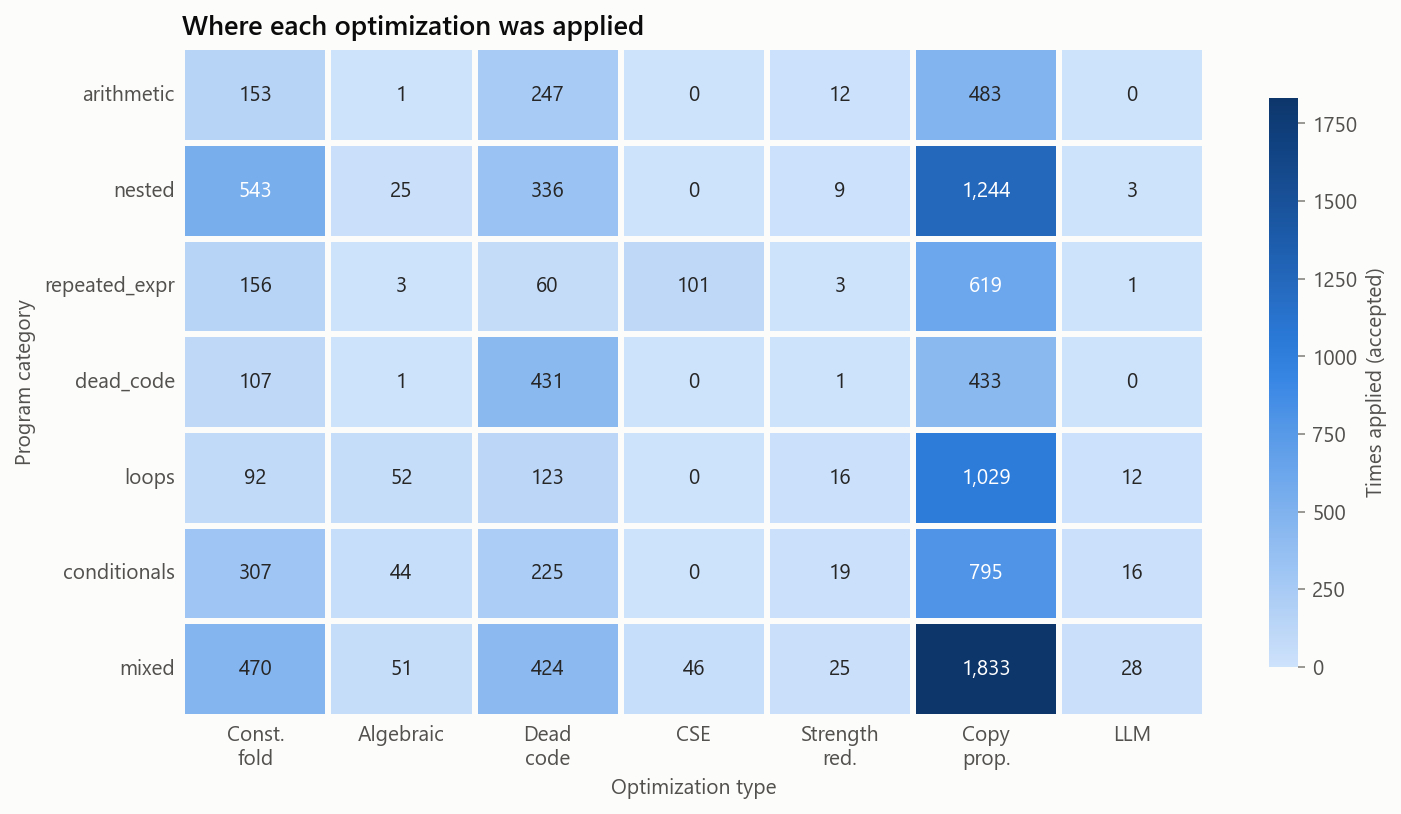
\includegraphics[width=\textwidth]{report_figures/heatmap_ollama.png}
\caption{Ollama run: accepted optimizations for each program category and optimization type}
\label{fig:heatmap-ollama}
\end{figure}

\section{Performance Analysis and Evaluation}

A few observations stand out from the numbers:

\textbf{The verifier works.} All 10,628 rule-based proposals passed verification; not one was incorrect. This is expected, since the rules are correct by construction, but it confirms that the verifier does not produce false rejections. On the LLM side, 26 of Gemini's 340 usable proposals (7.65\%), 6 of Groq's 318 (1.9\%) and 113 of the local model's 198 (57\%) were semantically wrong, and the verifier caught every single one. The false-positive count across all four runs is zero.

\textbf{Cost-neutral strength reductions get rejected, as intended.} Under our weight scheme, replacing \texttt{x * 2} with \texttt{x + x} swaps one arithmetic operation for another at the same cost. The evaluator rightly rejects these. Replacing \texttt{x * 4} with \texttt{x {<}{<} 2}, on the other hand, replaces an arithmetic operation (weight 2.0) with a non-arithmetic shift, so it is accepted. This accounts for 97 of the 111 rejections in the rule-only run.

\textbf{Copy propagation is the workhorse.} It accounts for about 60\% of all accepted changes because each high-priority transformation (a fold, a CSE, a dead-code removal) often creates new copies that need to be propagated and cleaned up. A single constant fold might trigger three or four subsequent copy-propagation steps.

\textbf{The LLM helps most where rules are structurally limited.} Rules cannot ``think about'' what a loop computes in aggregate. They can fold constants inside the body, but the loop control flow survives. An LLM can recognize that a loop with a constant trip count and a constant body evaluates to a single value, and it proposes the collapsed form. The verifier then confirms it on its test inputs. This pattern explains the 28-point jump in the loops category.

\textbf{A weak model is still safe.} The local model's low validity rate did not make the results worse, only slower. This is the main practical consequence of verifying every proposal: the choice of model affects how much is gained, never whether the result is correct.

\textbf{Convergence is fast.} The median program converges in 20 iterations (about 0.5 seconds rule-only). The full 500-program rule-only run finishes in under 2 minutes. With a cloud LLM the bottleneck is the pause between API calls, which the free tiers require, bringing the total to about 43 minutes. Both cloud providers also limit requests and tokens per day; the system spaces its calls, waits out per-minute limits, and for Groq moves to another model when one quota is spent, so a full run completes without supervision. The local model has no quota but took 2 hours 14 minutes on the laptop CPU.

\subsection{Limitations}

\begin{itemize}[leftmargin=2cm]
  \item The cost model is static: it counts instructions, arithmetic operations, temporaries, copies and branches. It does not measure execution time, so removing an instruction inside a loop is valued the same as removing one outside it.
  \item For programs with branches \emph{and} inputs, differential testing is thorough but is not a proof. Programs without inputs and straight-line programs are proven equivalent.
  \item The offline run used the CPU, because the local GPU driver was too old for the model runner. With a working GPU the same run should be several times faster.
  \item The dataset programs are small and generated. Larger, real-world programs remain future work.
\end{itemize}


% ============================================================
\newpage
\begin{center}
{\fontsize{16}{20}\selectfont \textbf{REFERENCES}}
\end{center}
\addcontentsline{toc}{chapter}{REFERENCES}
\vspace{0.3cm}

\setstretch{1.15}
\refgroup{Journals and Preprints:}

\apa{Chen, M., Tworek, J., Jun, H., Yuan, Q., Pinto, H. P., Kaplan, J., \ldots\ \& Zaremba, W. (2021). Evaluating large language models trained on code. \textit{arXiv preprint arXiv:2107.03374}.}

\apa{Cummins, C., Seeker, V., Grubisic, D., Roziere, B., Gehring, J., Synnaeve, G., \& Leather, H. (2024). Meta Large Language Model Compiler: Foundation models of compiler optimization. \textit{arXiv preprint arXiv:2407.02524}.}

\apa{Rozi\`ere, B., Gehring, J., Gloeckle, F., Sootla, S., Gat, I., Tan, X. E., \ldots\ \& Synnaeve, G. (2023). Code Llama: Open foundation models for code. \textit{arXiv preprint arXiv:2308.12950}.}

\apa{Wu, Q., Bansal, G., Zhang, J., Wu, Y., Li, B., Zhu, E., \ldots\ \& Wang, C. (2023). AutoGen: Enabling next-gen LLM applications via multi-agent conversation. \textit{arXiv preprint arXiv:2308.08155}.}

\refgroup{Conferences:}

\apa{Cummins, C., Wasti, B., Guo, J., Cui, B., Ansel, J., Gomez, S., \ldots\ \& Leather, H. (2022). CompilerGym: Robust, performant compiler optimization environments for AI research. \textit{Proceedings of the IEEE/ACM International Symposium on Code Generation and Optimization (CGO)}, 92--105.}

\apa{Lattner, C., \& Adve, V. (2004). LLVM: A compilation framework for lifelong program analysis \& transformation. \textit{Proceedings of the IEEE/ACM International Symposium on Code Generation and Optimization (CGO)}, 75--86.}

\apa{Massalin, H. (1987). Superoptimizer: A look at the smallest program. \textit{Proceedings of the 2nd International Conference on Architectural Support for Programming Languages and Operating Systems (ASPLOS)}, 122--126.}

\apa{Necula, G. C. (2000). Translation validation for an optimizing compiler. \textit{Proceedings of the ACM SIGPLAN Conference on Programming Language Design and Implementation (PLDI)}, 83--94.}

\apa{Phothilimthana, P. M., Thakur, A., Bodik, R., \& Dhurjati, D. (2016). Scaling up superoptimization. \textit{Proceedings of the 21st International Conference on Architectural Support for Programming Languages and Operating Systems (ASPLOS)}, 297--310.}

\apa{Pnueli, A., Siegel, M., \& Singerman, E. (1998). Translation validation. \textit{Proceedings of the International Conference on Tools and Algorithms for the Construction and Analysis of Systems (TACAS)}, 151--166.}

\refgroup{Books:}

\apa{Aho, A. V., Lam, M. S., Sethi, R., \& Ullman, J. D. (2006). \textit{Compilers: Principles, Techniques, and Tools} (2nd ed.). Pearson.}

\apa{Muchnick, S. S. (1997). \textit{Advanced Compiler Design and Implementation}. Morgan Kaufmann.}

\apa{Stallman, R. M., \& the GCC Developer Community. (2023). \textit{Using the GNU Compiler Collection (GCC 13)}. Free Software Foundation.}

\refgroup{Web links:}

\apa{Groq. (2026). \textit{GroqCloud API documentation}. https://console.groq.com/docs}

\apa{Ollama. (2026). \textit{Ollama: Run large language models locally}. https://ollama.com}

\end{document}
